\section{Analysis}\label{sec:analysis}

Section~\ref{sec:requirements} introduced a set of requirements to judge the
results of this work and Section~\ref{sec:objectives} introduced a set of
objectives this research targeted for completion. This section reviews those
sections in the context of test results produced for this work.

% This work, by virtue of building on an Internet-based network, is accepting
% risks which make any consideration or application of its results inappropriate
% for use in large-scale high-risk elections. Specifically, the intrinsically
% electronic and remote properties, which are inherent in all publicly-available
% ``off-the-shelf'' blockchain technologies, present so large an attack surface
% for would-be attackers that it becomes an untenable foundation for any voting
% systems being considered for use in elections where a high-risk threat model is
% maintained. Correctness, security, integrity, verifiability, and efficacy are
% the primary concerns of the systems designed and considered in this research;
% however, it is worth noting that the privacy constraints offered by traditional
% voting systems are severely loosened within the scope of this research: no
% notion of receipt-freedom is assumed and privacy is only guaranteed insofar as
% the pseudo-anonymity provided by the Ethereum blockchain is
% maintained.\footnotemark{}
%
% \footnotetext{
%   It is feasible that blockchain technologies could demonstrate utility in
%   large-scale voting systems if incorporated using well-established and
%   known-safe patterns: e.g., voter verifiable paper audit trails, private
%   networks, requiring transactions be signed by authorized sources, using voting
%   machines which have been certified by a federal commission, which are being
%   hosted in traditional polling locations, and are leveraging the appropriate
%   cryptographic techniques to ensure privacy; e.g., homomorphic encryption,
%   blind signing, and mix networks.
%
%   % The feasibility of leveraging fully- or partially-decentralized blockchains
%   % as a foundation for large-scale voting systems demands significantly more
%   % research into crypto-economic incentivization and disincentivization models
%   % for honest and dishonest actors.
%
%   % That said, the computational and storage requirements of such a project
%   % would almost certainly necessitate a dedicated blockchain solution.
% }

\subsection{Requirements}
Table~\ref{tab:research-requirements-fulfilled} highlights these requirements
targeted from Section~\ref{sec:requirements} and provides an overview of what
was and was not fulfilled. \\

\begin{spacing}{1.1}
  \begin{longtabu} to \textwidth{X[0.1,l] X[2.3,j] X[0.8,c] X[0.8,c] X[0.8,c] X[1.1,c]}
    % \multicolumn{2}{c}{Requirements} \\
    \caption{Requirements targeted for fulfillment.} \\
    \toprule
    \multicolumn{2}{l}{{Requirements}}                                       & \multicolumn{3}{c}{Fulfilled}                  & {Unfulfilled} \\
                                                                               \cmidrule{3-5}
    \multicolumn{2}{l}{}                                                     & {Fully}       & {Mostly}       & {Partially}   &               \\
    \midrule
    \endhead
    \multicolumn{2}{l}{\emph{Technical}} \\
    % \cmidrule(lr){1-2} \cmidrule(lr){3-5} \cmidrule(lr){6-6}
    % \cline{1-2}
    % \midrule
    % \multirow{10}{*}{\rot[90]{Technical}}     & Authentication               & \textbullet{} &                &               &               \\
                                              & Authentication               &               & \textbullet{}  &               &               \\
                                              & System Operational           & \textbullet{} &                &               &               \\
                                              & Reliability                  &               & \textbullet{}  &               &               \\
                                              & Security                     &               & \textbullet{}  &               &               \\
                                              & Auditing                     &               & \textbullet{}  &               &               \\
                                              & Functional                   &               & \textbullet{}  &               &               \\
                                              & Interoperability             &               &                & \textbullet{} &               \\
                                              & Certification                &               &                & \textbullet{} &               \\
                                              & Accessibility                &               &                &               & \textbullet{} \\
                                              & Usability                    &               &                &               & \textbullet{} \\
    % \midrule
    % \cmidrule(lr){1-2} \cmidrule(lr){3-5} \cmidrule(lr){6-6}
    \addlinespace[0.4ex]
    \cmidrule(lr){1-2} \cmidrule(lr){3-5} \cmidrule(lr){6-6}
    \multicolumn{2}{l}{\emph{Non-Functional}} \\
    % \cmidrule(lr){1-2} \cmidrule(lr){3-5} \cmidrule(lr){6-6}
    % \cline{1-2}
    % \cmidrule{1-2}
    % \midrule
    % \multirow{5}{*}{\rot[90]{Non-Functional}} & Maintenance/Evolvability     &               & \textbullet{}  &               &               \\
                                              & Maintenance/Evolvability     &               &                & \textbullet{} &               \\
                                              & Assurance                    &               &                & \textbullet{} &               \\
                                              & Operational                  &               &                &               & \textbullet{} \\
                                              & Procedural                   &               &                &               & \textbullet{} \\
                                              & Legal                        &               &                &               & \textbullet{} \\
    \bottomrule\label{tab:research-requirements-fulfilled}
  \end{longtabu}
\end{spacing}

\subsubsection{Technical Requirements}
The technical requirements are ones which are meant to be fulfilled through the
design and architecture of the system. The system operational requirements are
considered fulfilled here. The functional and audibility requirements were
fulfilled as expected. The accessibility and usability requirements were not
targeted.

\paragraph{Certification}
The certification requirements assert that proofs of correctness are necessary,
which this research falls short of, but the tests and documentation available do
fulfill other certification requirements listed.

\paragraph{Authentication}
This research deeply explored authentication models and techniques for managing
access control for use in constructing voter registries. Much of this research
focused on building systems which would be reusable and composable across many
election and non-election systems; however, the result of these access control
models produced a security interface that, although working, is difficult to
interact with in a reasonable way. Inter-contract communication is difficult and
managing locks and mutexes across them is even more-so. Managing a security
interface which is entirely or mostly internal to a single contract is likely a
much safer approach to consider in most cases, although probably also a less
flexible model in the long-term. However, a majority of the most important
authentication functionalities required are provided through the underlying
blockchain infrastructure.

\paragraph{Reliability Requirements}
The underlying resiliency of the Ethereum network provides strong reliability
guarantees; however, the network is not without its issues and has seen attacks
on it over time. More recently the network has faced serious scaling issues
which have driven gas prices up and made smart contract operation an expensive
endeavour.

\paragraph{Security Requirements}
This work, by virtue of building on an Internet-based network, is accepting
risks which make any consideration or application of its results inappropriate
for use in large-scale high-risk elections. Specifically, the intrinsically
electronic and remote properties, which are inherent in all publicly-available
``off-the-shelf'' blockchain technologies, present so large an attack surface
for would-be attackers that it becomes an untenable foundation for any voting
systems being considered for use in elections where a high-risk threat model is
maintained. Correctness, security, integrity, verifiability, and efficacy are
the primary concerns of the systems designed and considered in this research;
however, it is worth noting that the privacy constraints offered by traditional
voting systems are severely loosened within the scope of this research: no
notion of receipt-freedom is assumed and privacy is only guaranteed insofar as
the pseudo-anonymity provided by the Ethereum blockchain is maintained.

It is feasible that blockchain technologies could demonstrate utility in
large-scale voting systems if incorporated using well-established and known-safe
patterns: e.g., voter verifiable paper audit trails, private networks, requiring
transactions be signed by authorized sources, using voting machines which have
been certified by a federal commission, which are being hosted in traditional
polling locations, and are leveraging the appropriate cryptographic techniques
to ensure privacy; e.g., homomorphic encryption, blind signing, and mix
networks.

\subsubsection{Non-Functional Requirements}
The non-functional requirements as described in Section~\ref{sec:requirements}
are only fulfilled insofar as this document and source code exists. Strong
efforts were not otherwise made to fulfill these requirements.

\subsection{Objectives}
Section~\ref{sec:objectives} introduced a set of objectives this research
targeted for completion. This research succeeded in exploring electoral system
design and implementation and produced several contracts demonstrating
single-winner electoral systems. However, this failed to implement a
multi-winner electoral system supporting proportional representation. STV is
often described as a complex to implement electoral system with difficult to
handle edge-cases. The finite storage and computational resources made available
by the EVM make it a poor candidate for exploration. There are other
proportional representation systems with much lower storage and execution
complexities which are probably better candidates for resource-constrained
environments like smart contracts.

This research thoroughly explored and designed many voter authentication,
registration, and access control patterns for voter registration. However, as
previously stated, inter-contract communication is difficult to manage,
especially when multiple contracts might be deferring responsibility to a single
contract managing state. This issue, combined with the resource constraints of
smart contracts, is ultimately what made further research into delegative or
liquid governance models infeasible. There are too many inter-contract
communication issues to manage when attempting to compute delegations across
contracts and there does not appear to be any clear way of designing smart
contract dependencies in a way which enabled them to be open to state changes
while still providing consistent values during sensitive contract execution
procedures like ballot tabulation or delegation analysis.

% 1. This research aims to explore various electoral systems and features, using the
% content reviewed in Section 2.1 as a basis for exploration.
% (a) Provide a range of kinds of electoral contracts using Table 2.1 and Table 2.2
% as the primary resource for electoral system and feature selection.
% i. Support single-winner elections and provide plurality and majority elec-
% toral system in fulfillment of that objective.
% A. Implement first-past-the-post to fulfill the targeted single-winner
% plurality electoral system, due mostly to the fact that it is extremely
% simple, well-understood, and widely-adopted.
% B. Implement range vote to fulfill the targeted single-winner majority
% electoral system, due to its effectiveness and simplicity.
% ii. Support multi-winner elections and provide an electoral system which
% offers proportional representation; Single transferable vote is selected as
% the electoral system implementation to fulfill both objectives due to its
% 89wide-adoption, prevalence, and effectiveness as a PR system.
% (b) Explore the design, implementation, and efficacy of various ballot types
% across the various electoral systems selected.
% 2. This research aims to explore voter authentication, registration, and access control
% patterns for managing voter registration.
% 3. This research aims to explore delegative or liquid governance models.
% 86Auditability Requirements Ethereum inherently offers a tremendously detailed
% log through its blockchain structure which provides a wide range of opportunities for
% detailed auditing and validation. Furthermore, auditing and validation functionality
% are inherent features of the blockchain. However, the auditability which Ethereum
% provides is not considered a privacy preserving feature and therefore falls short of
% the criteria presented.
% Functional Requirements A subset of the functional requirements are deemed
% relevant to this research:
%  Multi-vote functionality is targeted to be investigated and fully satisfied in all
% electoral system implementations.
% + Ensuring that “a voter’s ballot, and the act of them casting a ballot, is recorded
% and retained as expected;” is considered mostly fulfilled through intrinsic prop-
% erties of the Ethereum blockchain. Where this property falls short is when a
% voter casts a ballot, broadcasts a transaction to the network, which miners fail
% to include in any blocks. This is discussed further in Chapter 6, Discussion.
% − Maintaining voter anonymity is considered partially fulfilled through intrin-
% sic properties of the Ethereum blockchain. While it is technically possible to
% broadcast privacy-maintaining transactions, those which preserve anonymity
% on the Ethereum network, it is likely beyond the capabilities of most voting
% 87actors and would be difficult to guarantee in any meaningful way. Pseudo-
% anonymity is a better profile of the kind of anonymity whic

% \input{05-results/example}

% \blockquote{
%     Arrow assumed that social orderings will be derived, if at all, from information
%     about people's preferences. This information is, in his framework, merely
%     ordinal. It is the kind of information that is implicated in Condorcet's paradox
%     of voting, in Section 1, where each person ranks the alternatives from better to
%     worse but there is nothing beyond this about how strong anybody's preferences
%     are, or about how the preferences of one person compare in strength to those of
%     another. In confining aggregation procedures to ordinal information, Arrow
%     argued that:
%
%     [I]t seems to make no sense to add the utility of one individual, a psychic
%     magnitude in his mind, with the utility of another individual. (Arrow 1951
%     [1963]: 11)
%
%     His point was that even if people do have stronger and weaker preferences, and
%     even if the strengths of their preferences can somehow be measured and made
%     available as a basis for social decisions, nevertheless ordinal information is
%     all that matters because preferences are “interpersonally incomparable”.
%     Intuitively, what this means is that there is no saying how much more strongly
%     someone must prefer one thing to another in order to make up for the fact that
%     someone else's preference is just the other way around. Arrow saw no reason to
%     provide aggregation procedures with information about the strength of
%     preferences because he thought that they cannot put such information to
%     meaningful use.
% }

% Section: Authorization Components
% \section{Authorization Components}

The authorization components are those which are responsible for managing access
control for \solt{contract}[s]. This section builds varying complexities of
access control beginning with:

\begin{enumerate}
  \item \emph{Primitive Contract Ownership}, which reviews basic access control
    mechanisms; then

  \item \emph{Generalized Access Control}, which introduces components for
    guarding access to resources; next

  \item \emph{Access Control Lists}, which demonstrate components for
    constructing and managing access control lists and integrating them with the
    components introduced for generalized access control; and finally,

  \item \emph{Registries}, which demonstrates voter registry components
    leveraging the aforementioned components to build and manage voter
    databases.
\end{enumerate}

\begin{figure}[H]
  \centering
  \caption{Authorization dependency graph modeling.}% \label{fig:authorization}
  \figurepdf[width=\textwidth]{authorization}
  % 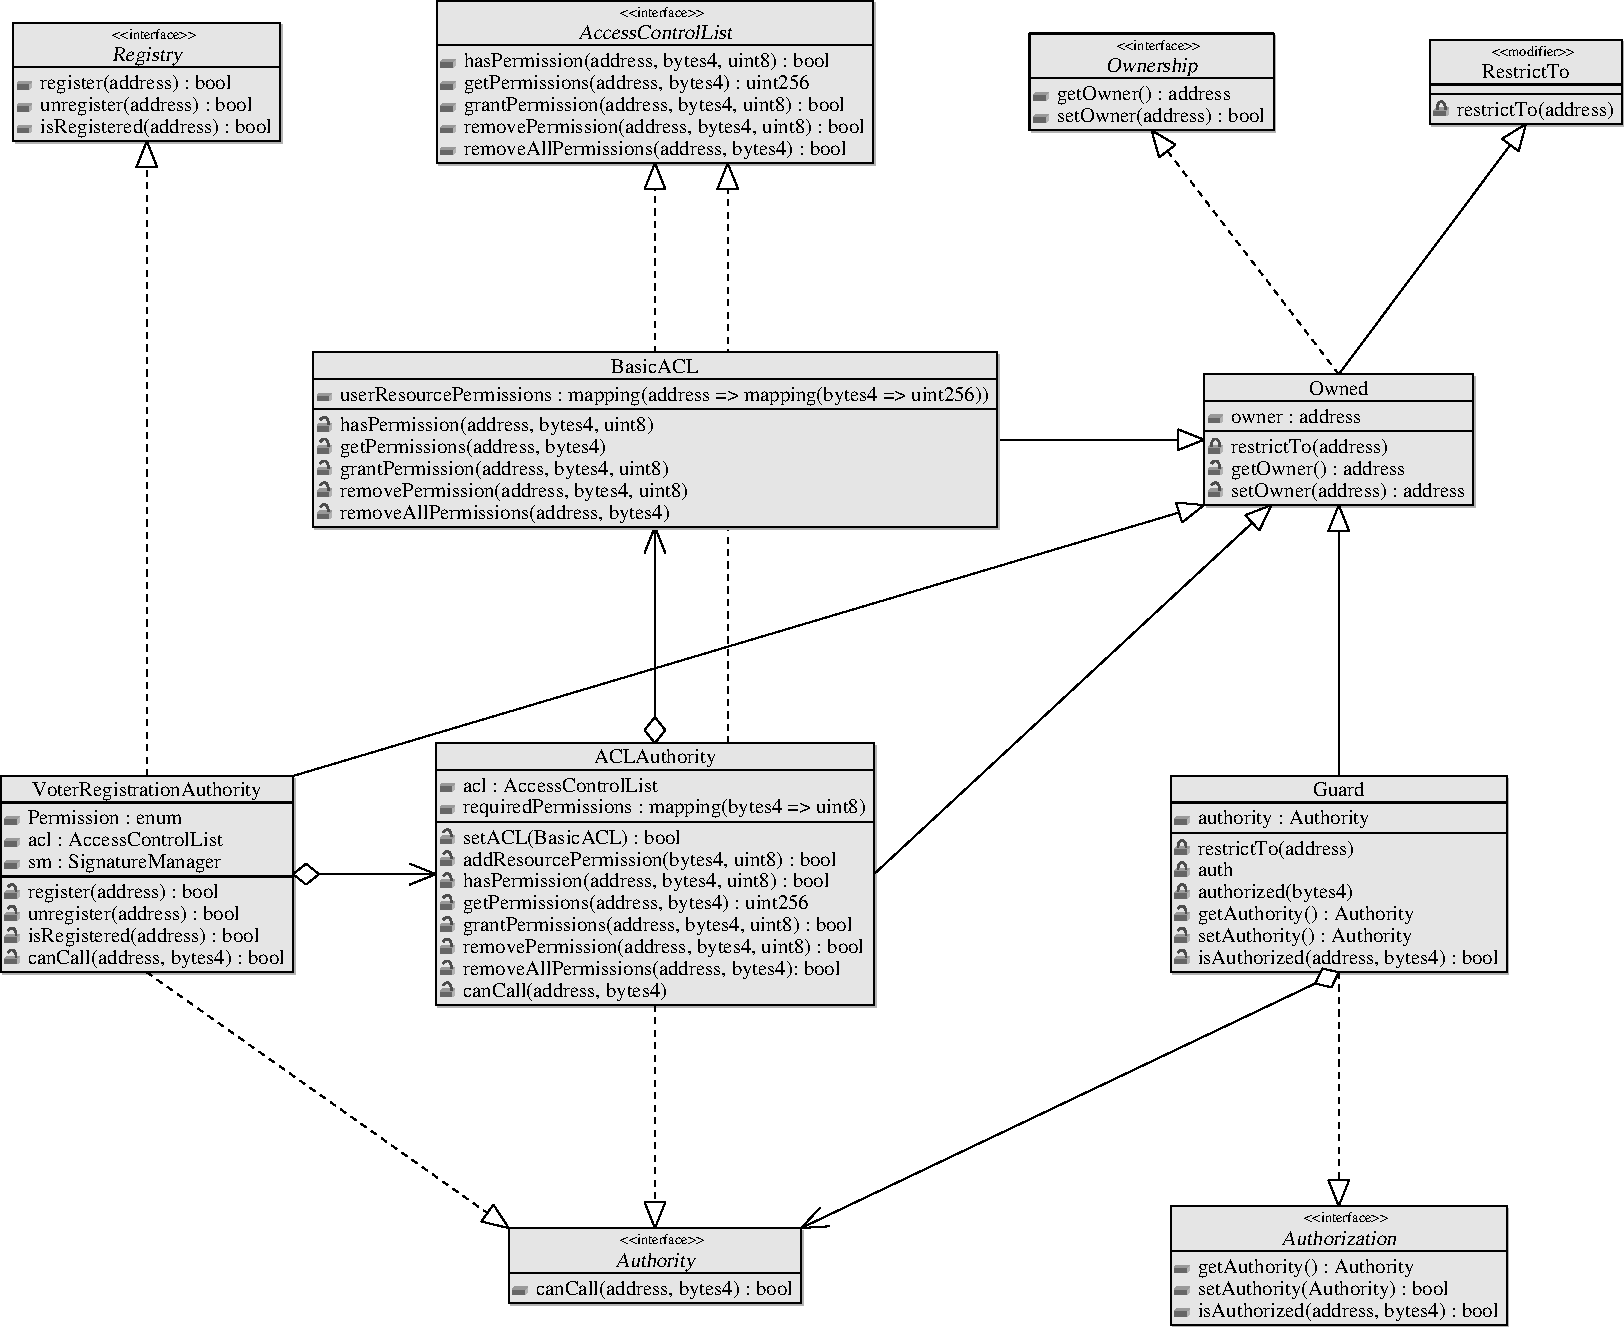
\includegraphics[width=\textwidth]{figures/authorization/figure}
  % \includestandalone[width=\textwidth]{\fig{authorization}}
\end{figure}

% Sub-sub-section: Managing Contract Ownership
\subsection{Primitive Contract Ownership}

Managing \solt{contract} ownership is one of the most basic forms of access
control in the Ethereum ecosystem. Here we introduce:

\begin{enumerate}
  \item \sol{interface Ownership}, which defines \solt{function}[s] to
    express \solt{contract} ownership,
  \item \sol{contract RestrictTo}, which defines a \solt{modifier} for
    restricting access to \solt{function} calls based on an \solt{address}, and
  \item \sol{contract Owned}, a convenience \solt{contract}, which provides an
    implementation of \sol{interface Ownership} and leverages
    \sol{contract RestrictTo}.
\end{enumerate}

\begin{figure}[H]
  \centering
  \caption{Contract ownership dependency graph modeling.}\label{fig:ownership}
  \figurepdf[]{ownership}
\end{figure}

\subsubsection{Contract RestrictTo}

The \solt{contract}, \sol{contract RestrictTo}, introduces a single
\solt{modifier}, \sol{modifier restrictTo}, which requires the caller of the
\solt{function}, \sol{msg.sender}, to have the same \solt{address} as the
argument, \sol{address _subject}, provided to the \solt{modifier} when called.

\begin{solidity}[contract RestrictTo]
contract RestrictTo {
  modifier restrictTo (address _subject) {
    require(msg.sender == _subject);
    _;
  }
}
\end{solidity}

\begin{code}
  \item \operations
  \begin{modifiers}
    \item \sol{modifier restrictTo (address _subject)}, restricts access to
      \solt{function} calls based on an \solt{address} provided.

      \begin{displayquote}
        Restriction to \solt{function}[s] is accomplished by comparing the
        \solt{address} of the \solt{function} \emph{caller}, \sol{msg.sender},
        against the configured \solt{address}, \sol{address _subject}. If the
        \solt{address} of the \solt{msg.sender} does not match the
        \solt{address} of the \solt{_subject} then the \solt{require} statement
        will force the immediately arrest of \solt{contract} evaluation,
        \solt{revert} the \emph{state} of the \solt{contract}, refund any
        remaining \solt{gas}, \solt{gasleft()}, to the \emph{caller}, and
        exit.\footnotemark{}

        \todo{Should notes be documented differently?}
      \end{displayquote}

      \footnotetext{
        Note that the \emph{caller}, \sol{msg.sender}, of the \solt{function}
        will not necessarily be an \emph{external account}, e.g., human user;
        the \emph{caller} of the \solt{contract} \solt{function} may itself also
        be a \solt{contract}, i.e., a \emph{contract account}, which is calling
        the \solt{contract} \solt{function} from its own \solt{contract}
        \solt{function}.
      }

      \begin{parameters}
      \item \sol{address _subject}, the \emph{subject} who is to be granted
        access to the \solt{function}.

        \begin{displayquote}
          The \solt{address} of the \emph{subject} may be \emph{any} Ethereum
          account, including \emph{contract accounts}.
        \end{displayquote}
      \end{parameters}
  \end{modifiers}
\end{code}


\paragraph{Interface Ownership}

The \solt{interface}, \sol{interface Ownership}, introduces two
\solt{function}[s] for managing contract ownership:

\begin{enumerate}
  \item \sol{function getOwner}, which is expected to return the \solt{address}
        of the owner of the \solt{contract}, and
  \item \sol{function setOwner}, which is expected to update the \solt{address}
        of the owner of the \solt{contract}.
\end{enumerate}

\begin{solidity}[interface Ownership]
interface Ownership {
  function getOwner () public view returns (address _owner);
  function setOwner (address _owner) public returns (bool _success);
}
\end{solidity}

\begin{interface}
\item \specification{}

  \begin{functions}
    \item \sol{function getOwner ()}, returns the \solt{address} of the owner of
      the \solt{contract}.

      \begin{returns}
        \item \sol{address _owner}, the \emph{subject} representing the owner of
          the \solt{contract}.
      \end{returns}

    \item \sol{function setOwner (address _owner)}, updates the \solt{address}
      representing the owner of the \solt{contract}.

      % which accepts an \solt{address},
      % \sol{address _owner}, and is expected to update the owner of the
      % \solt{contract} and \solt{return} a \solt{bool}, \sol{bool _success},
      % which resolves to \solt{true} if the operation was successful; otherwise
      % \solt{false}.


      \begin{parameters}
      \item \sol{address _owner}, the \emph{subject} which is to be granted
        ownership of the \solt{contract}.\footnotemark{}

        \footnotetext{\label{param:address-owner}
          The \solt{address} of the \emph{subject} may be \emph{any} Ethereum
          account, including \emph{contract accounts}.
        }
      \end{parameters}

      \begin{returns}
      \item \sol{bool _success}, resolves to \solt{true} if the operation was
        successful; otherwise \solt{false}.
      \end{returns}
  \end{functions}
\end{interface}


\subsubsection{Contract Owned}

A convenience \solt{contract}, \sol{contract Owned}, implements
\sol{interface Ownership} and extends \sol{contract RestrictTo}; in doing so,
\sol{contract Owned} provides a simple mechanism for expressing \solt{contract}
ownership, extending \sol{contract Owned}; e.g., \sol{contract MyContract is
Owned {}}.

% Upon creation, the \solt{constructor} of this \solt{contract} sets the
% \solt{owner} property of the \solt{contract} to the \solt{address} which
% created the contract, and restricts future calls to the \sol{function
% setOwner} to the owner of the \solt{contract} by using the \sol{modifier
% restrictTo(owner)}.

\begin{solidity}[contract Owned]
contract Owned is RestrictTo, Ownership {
  address public owner;

  constructor () {
    owner = msg.sender;
  }

  function getOwner () public view returns (address _owner) {
    return owner;
  }

  function setOwner (address _owner) public restrictTo(owner) returns (bool _success) {
    owner = _owner;
    return true;
  }
}
\end{solidity}

\begin{state}
  \item \attributes

  \begin{public}
    \item \sol{address owner}, maintains the \solt{address} of the current
      \solt{owner} of the \solt{contract}.
  \end{public}
\end{state}

\begin{code}
  \item \operations

  \begin{constructor}
    \item \sol{constructor ()}, upon creation and initialization of this
      \solt{contract} the \solt{constructor} sets the \sol{address owner}
      property of the \solt{contract} to the \solt{address} of the
      \solt{contract} creator, \sol{msg.sender}, i.e., the \emph{subject}
      submitting the \solt{CREATE} opcode.
  \end{constructor}

  \begin{functions}
    \item \sol{function getOwner ()}, returns the \solt{address} of the owner of
      the \solt{contract}.

      \begin{returns}
        \item \sol{address _owner}, the \emph{subject} representing the owner of
          the \solt{contract}.
      \end{returns}

    \item \sol{function setOwner (address _owner)}, updates the \solt{address}
      representing the owner of the \solt{contract}, effectively transferring
      ownership of the \solt{contract}.

      \begin{modifiers}
        \item \sol{modifier restrictTo (owner)}, restricts access to the
          \solt{function} such that \emph{only} the current \solt{owner} of the
          \solt{contract} can update/transfer ownership of the \solt{contract}.
      \end{modifiers}

      \begin{parameters}
        \item \sol{address _owner}, the \emph{subject} who is to be granted access
          to the \solt{function}.
      \end{parameters}

      \begin{returns}
        \item \sol{bool _success}, the \emph{subject} representing the owner of
          the \solt{contract}
      \end{returns}
  \end{functions}
\end{code}


% Sub-sub-section: Generalizing Contract Access Control
\subsection{Generalizing Contract Access Control}

In order to generalize \solt{contract} access control we introduce:

\begin{enumerate}
  \item \sol{interface Authority}, which defines \solt{function}[s] to determine
    whether some \emph{subject} is permitted to access some \emph{resource},
  \item \sol{contract Authorization}, which defines a \solt{modifier} for
    restricting access to \solt{function} calls based on an \solt{address}, and
  \item \sol{contract Guard}, a convenience \solt{contract}, which provides an
    implementation of \sol{interface Authorization} by aggregating
    implementations of \sol{interface Authority}.
\end{enumerate}

Together these components allow us to provide a generalized access control
model; isolating and deferring the responsibilities of
authorization.\footnotemark{}
\todo{Alternative names: Guard, Authority, Enforcer, Authorization}

\footnotetext{
  I think I would maybe prefer \sol{interface Authorization} to define
  \sol{isAuthorized} and for \sol{interface Authority} to define
  \sol{getAuthority} and \sol{setAuthority}.

  A better name in that case might be \sol{interface AuthorityManager}.
}

\begin{figure}[H]
  \centering
  \caption{Generalized contract access control.}% \label{fig:authorization}
  \figurepdf[]{guard}
  % 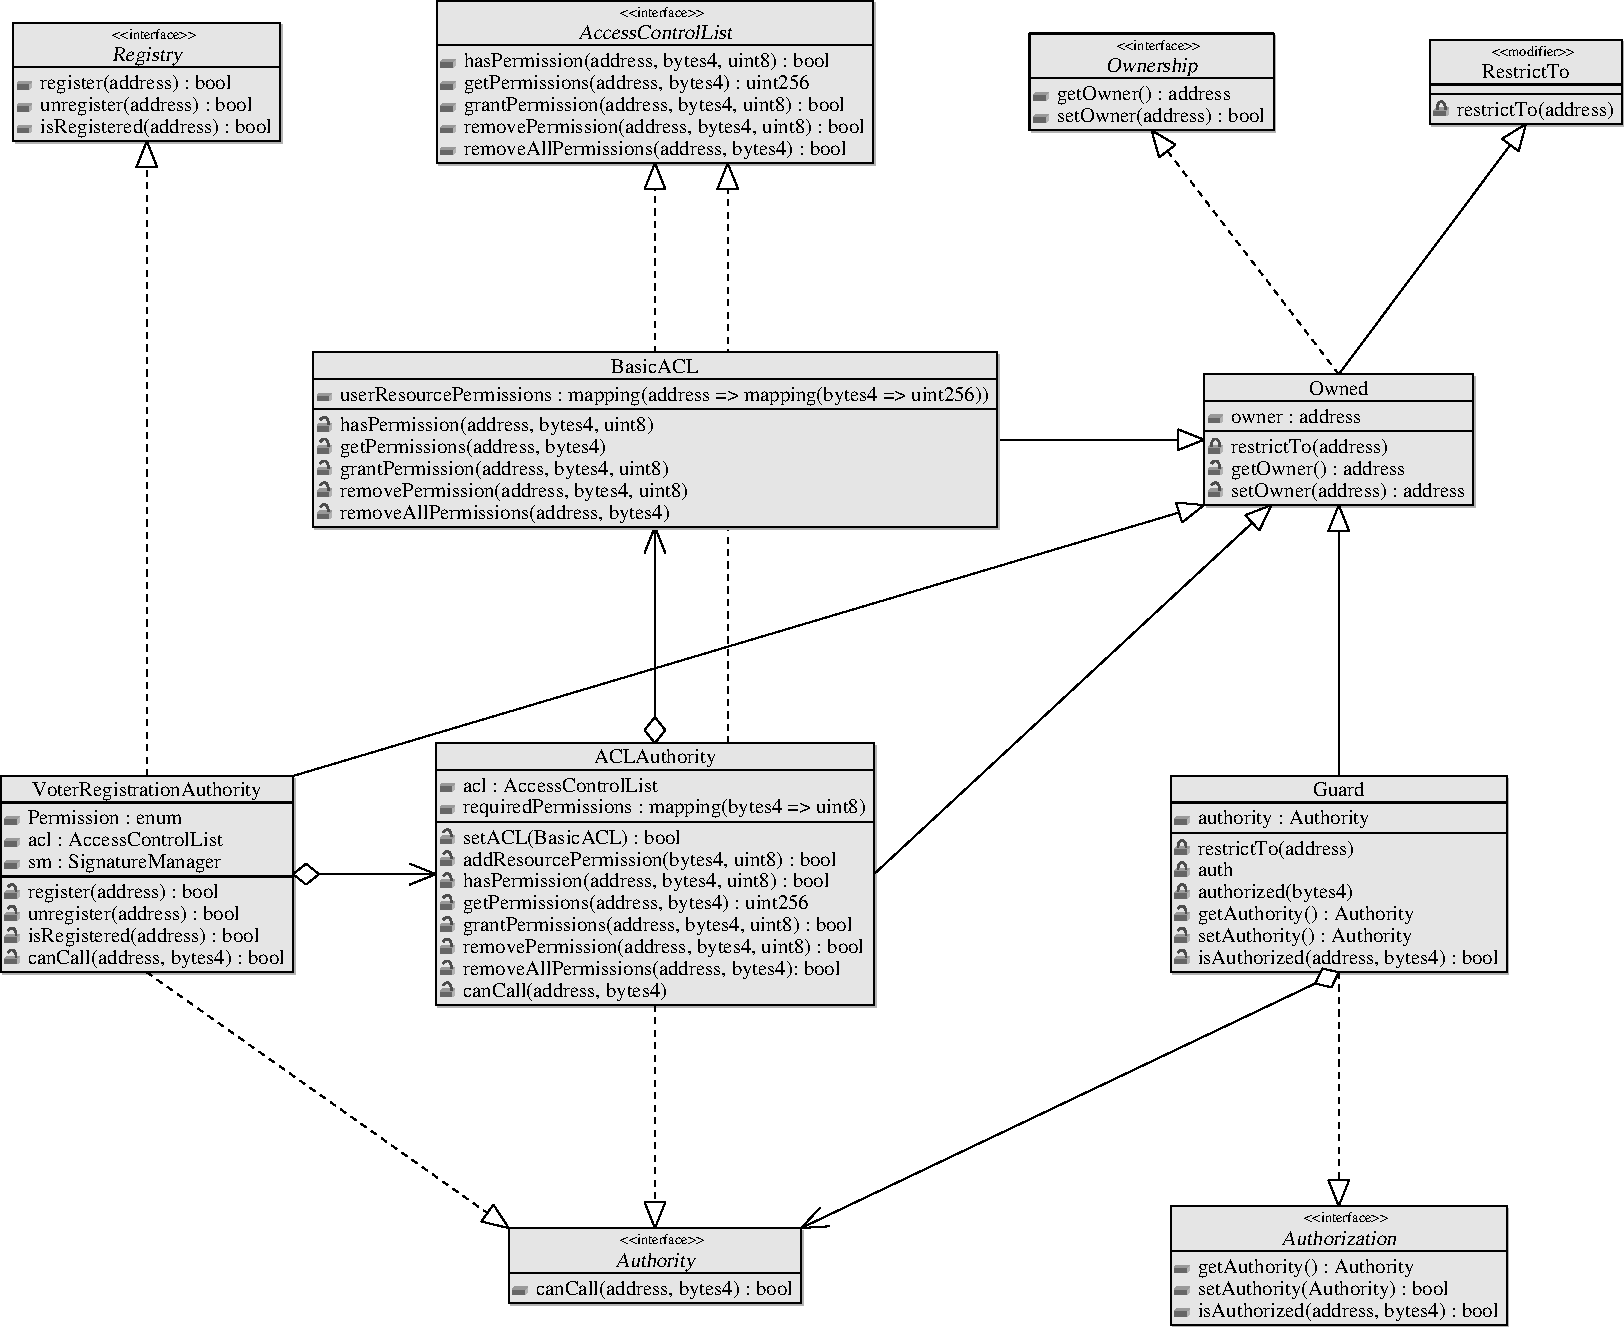
\includegraphics[width=\textwidth]{figures/authorization/figure}
  % \includestandalone[width=\textwidth]{\fig{authorization}}
\end{figure}

\subsubsection{Interface Authority}

The \solt{interface}, \sol{interface Authority}, introduces functionality for
managing whether some \emph{subject}, typically an Ethereum account represented
by \solt{address}, can access some \emph{resource}, typically an Ethereum
\solt{function} represented by \solt{function} signature, \solt{bytes4}. By
defining the \emph{resource} by it's \solt{function} signature and not by a
specific \solt{function} owned by a specific \solt{contract} we leave open the
possibility for managing \solt{contract} access control across
\solt{contract}[s], a functionality which will be necessary to build
pseudo-centralized registration authorities.

\begin{solidity}[interface Authority]
interface Authority {
  function canCall (address _subject, bytes4 _resource) public constant returns (bool _canCall);
}
\end{solidity}

\begin{interface}
  \item \specification{}

  \begin{functions}
    \item \sol{function canCall (address _subject, bytes4 _resource)}, evaluates
      whether some \emph{resource}, \solt{contract function}, can be used by
      some \emph{subject}, Ethereum account.

      \begin{parameters}
        \item \sol{address _subject}, the \emph{subject}, Ethereum account,
          whose permissions are being evaluated.\footnotemark{}

          \footnotetext{
            The \solt{address} of the \emph{subject} may be \emph{any} Ethereum
            account, including \emph{contract accounts}.
          }

        \item \sol{bytes4 _resource}, the \emph{resource}, \solt{contract
          function}, which the \emph{subject's} permissions are being evaluated
          against.
      \end{parameters}

      \begin{returns}
        \item \sol{bool _canCall}, resolves to \solt{true} if the
          \emph{subject}, \sol{address _subject}, is permitted to access the
          \emph{resource}, \sol{bytes4 _resource}, otherwise \solt{false}.
      \end{returns}
  \end{functions}
\end{interface}


\subsubsection{Interface Authorization}

The \solt{interface}, \sol{interface Authorization}, introduces functionality
for managing authorities, \sol{function getAuthority()} and \sol{function
setAuthority()}, and also functionality similar to that of an \solt{Authority},
\sol{function isAuthorized()}.\footnotemark{}

\footnotetext{
  If I don't update this to just be \sol{interface AuthorityManager} then I
  should \emph{really} update \sol{interface Authority} to supply \sol{function
  isAuthorized ()}, instead of \sol{function canCall()}, and update this
  \solt{interface} to implement/extend \sol{interface Authority}.
}

\begin{solidity}[interface Authorization]
interface Authorization {
  function getAuthority () public constant returns (address _authority);
  function setAuthority (address _authority) public returns (bool _success);
  function isAuthorized (address _subject, bytes4 _resource) public returns (bool _isAuthorized);
}
\end{solidity}

\begin{interface}
\item \specification{}

  \begin{functions}
    \item \sol{function getAuthority ()}, returns the \solt{address} of a
      \solt{contract} which implements the \solt{interface Authority}.

      \begin{returns}
        \item \sol{address _authority}, the \solt{address} of a \solt{contract}
          which implments the \solt{interface Authority}.
      \end{returns}

    \item \sol{function setAuthority (address _authority)}, updates the state of
      the \solt{contract} to to reflect the new \solt{contract} which provides
      an implementation of the \solt{Authority interface}.

      \todo{Make sure the Guard checks that the contract actually implements the
      interface!!!}

      \begin{parameters}
        \item \sol{address _authority}, the \solt{address} of a \solt{contract}
          which implements the \solt{interface Authority}.
      \end{parameters}

      \begin{returns}
        \item \sol{bool _success}, resolves to \solt{true} if the operation was
          successful; otherwise \solt{false}.
      \end{returns}

    \item \sol{function isAuthorized (address _subject, bytes4 _resource)},
      evaluates whether some \emph{subject}, Ethereum account, is authorized to
      access some \emph{resource}, \solt{contract function}.

      \begin{parameters}
        \item \sol{address _subject}, the \emph{subject}, Ethereum account,
          whose permissions are being evaluated.\footnotemark{}

          \footnotetext{
            The \solt{address} of the \emph{subject} may be \emph{any} Ethereum
            account, including \emph{contract accounts}.
          }

        \item \sol{bytes4 _resource}, the \emph{resource}, \solt{contract
          function}, which the \emph{subject's} permissions are being evaluated
          against.
      \end{parameters}

      \begin{returns}
        \item \sol{bool _isAuthorized}, resolves to \solt{true} if the
          \emph{subject}, \sol{address _subject}, is permitted to access the
          \emph{resource}, \sol{bytes4 _resource}, otherwise \solt{false}.
      \end{returns}
  \end{functions}
\end{interface}


\subsubsection{Contract Guarded}

The \solt{contract}, \sol{contract Guarded}, is a \solt{contract} which offers a
convenient mechanism for easily integrating generalized \solt{contract} access
control functionality; e.g., \sol{contract MyContract is Guarded {}}.
\solt{contract Guarded}, by virtue of implementing the \solt{Authorization
interface}, supports deferring access control responsibilities to an external
\solt{contract} which implements the \solt{Authority interface} while leaving
open the possibility for a \solt{contract} to provide its own access control
implementation by itself implementing the \solt{Authority interface}.

\todo{If I'm changing this from Guard to Guarded then I need to update all of
the references to Guard.}

\begin{solidity}[contract Guarded]
contract Guarded is Owned, Authorization {
  Authority public authority;

  function getAuthority () public constant returns (address _authority) {
    return address(authority);
  }

  function setAuthority (address _authority) public auth returns (bool _success) {
    authority = Authority(_authority);
    return true;
  }

  function isAuthorized (address _subject, bytes4 _resource) public returns (bool _isAuthorized) {
    if (_subject == address(this)) return true;
    if (authority == Authority(0)) return false;
    if (_subject == owner) return true;
    return authority.canCall(_subject, _resource);
  }

  modifier auth {
    assert(isAuthorized(msg.sender, msg.sig));
    _;
  }

  modifier authorized (bytes4 _resource) {
    assert(isAuthorized(msg.sender, _resource));
    _;
  }
}
\end{solidity}

\begin{code}
  \item \operations
  \begin{modifiers}
    \item \sol{modifier auth ()}, restricts access to \solt{function} calls
      based on an \solt{address} provided.

      \begin{displayquote}
        Restriction to \solt{function}[s] is accomplished by comparing the
        \solt{address} of the \solt{function} \emph{caller}, \sol{msg.sender},
        against the configured \solt{address}, \sol{address _subject}. If the
        \solt{address} of the \solt{msg.sender} does not match the
        \solt{address} of the \solt{_subject} then the \solt{require} statement
        will force the immediately arrest of \solt{contract} evaluation,
        \solt{revert} the \emph{state} of the \solt{contract}, refund any
        remaining \solt{gas}, \solt{gasleft()}, to the \emph{caller}, and
        exit.\footnotemark{}

        \todo{Should notes be documented differently?}
      \end{displayquote}

      \footnotetext{
        Note that the \emph{caller}, \sol{msg.sender}, of the \solt{function}
        will not necessarily be an \emph{external account}, e.g., human user;
        the \emph{caller} of the \solt{contract} \solt{function} may itself also
        be a \solt{contract}, i.e., a \emph{contract account}, which is calling
        the \solt{contract} \solt{function} from its own \solt{contract}
        \solt{function}.
      }

      \begin{parameters}
      \item \sol{address _subject}, the \emph{subject} who is to be granted
        access to the \solt{function}.

        \begin{displayquote}
          The \solt{address} of the \emph{subject} may be \emph{any} Ethereum
          account, including \emph{contract accounts}.
        \end{displayquote}
      \end{parameters}

    \item \sol{modifier authorized (address _resource)}, restricts access to
      \solt{function} calls based on an \solt{address} provided.

      \begin{displayquote}
        Restriction to \solt{function}[s] is accomplished by comparing the
        \solt{address} of the \solt{function} \emph{caller}, \sol{msg.sender},
        against the configured \solt{address}, \sol{address _subject}. If the
        \solt{address} of the \solt{msg.sender} does not match the
        \solt{address} of the \solt{_subject} then the \solt{require} statement
        will force the immediately arrest of \solt{contract} evaluation,
        \solt{revert} the \emph{state} of the \solt{contract}, refund any
        remaining \solt{gas}, \solt{gasleft()}, to the \emph{caller}, and
        exit.\footnotemark{}

        \todo{Should notes be documented differently?}
      \end{displayquote}

      \footnotetext{
        Note that the \emph{caller}, \sol{msg.sender}, of the \solt{function}
        will not necessarily be an \emph{external account}, e.g., human user;
        the \emph{caller} of the \solt{contract} \solt{function} may itself also
        be a \solt{contract}, i.e., a \emph{contract account}, which is calling
        the \solt{contract} \solt{function} from its own \solt{contract}
        \solt{function}.
      }

      \begin{parameters}
      \item \sol{address _subject}, the \emph{subject} who is to be granted
        access to the \solt{function}.

        \begin{displayquote}
          The \solt{address} of the \emph{subject} may be \emph{any} Ethereum
          account, including \emph{contract accounts}.
        \end{displayquote}
      \end{parameters}
  \end{modifiers}
\end{code}


% Sub-sub-section: Access Control Lists
\subsection{Access Control Lists}

We introduce access control lists to provide a generalized form of access
control through a well-understood and common interface:

\begin{enumerate}
  \item \sol{interface AccessControlList}, which defines the basic actions
    required for an access control list implementation;

  \item \sol{contract BasicACL}, which provides a basic implementation of
    \sol{interface AccessControlList}; and

  \item \sol{contract ACLAuthority}, which aggregates an
    \solt{interface AccessControlList} implementation, \sol{contract BasicACL}
    in this case, to back an \sol{interface Authority} implementation.
\end{enumerate}

\begin{figure}[H]
  \centering
  \caption{Generalized contract access control by way of access control lists.}\label{fig:acl}
  \figurepdf[]{access-control-lists}
  % 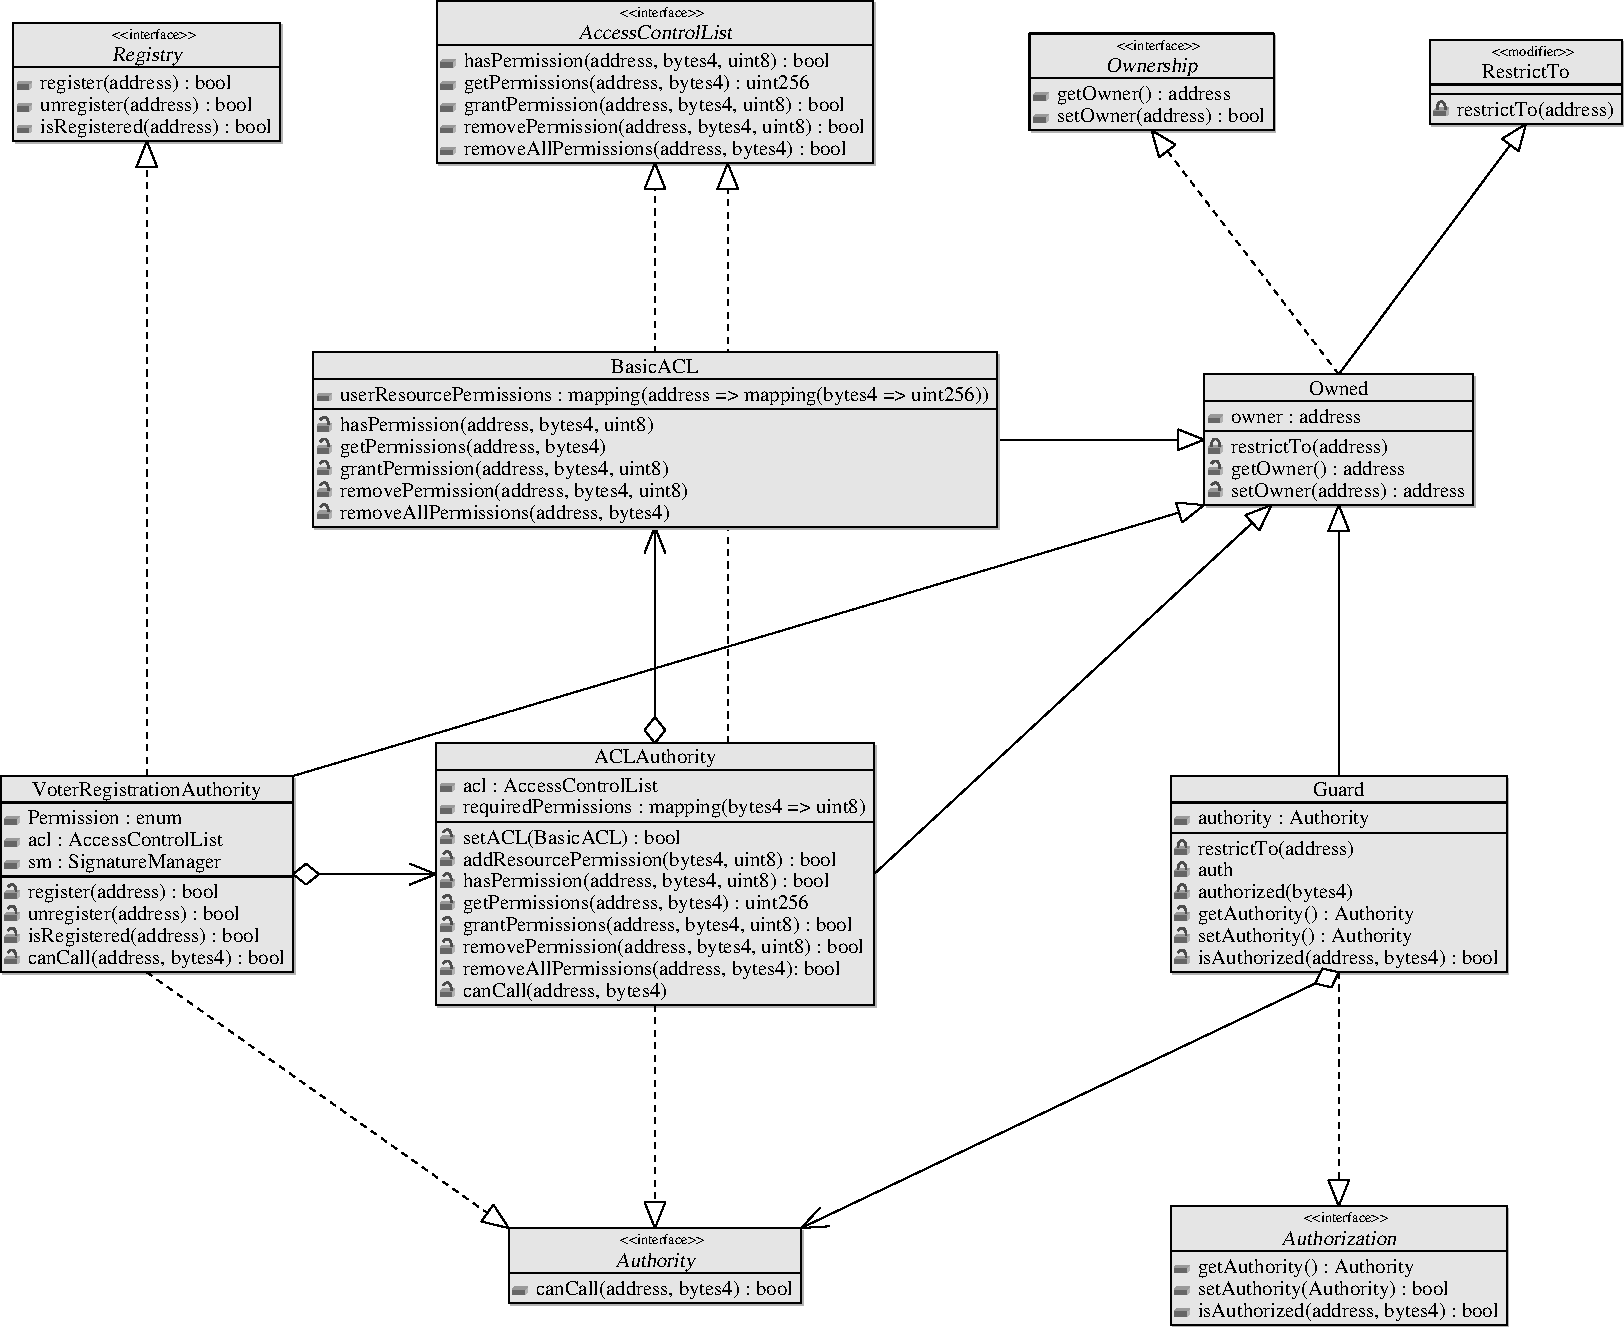
\includegraphics[width=\textwidth]{figures/authorization/figure}
  % \includestandalone[width=\textwidth]{\fig{authorization}}
\end{figure}

\subsubsection{Interface AccessControlList}

The \solt{interface}, \sol{interface AccessControlList}, introduces five
\solt{function} definitions to achieve basic access control list functionality:

\begin{enumerate}
  \item \sol{function hasPermission}, which validates that a \emph{subject} has
    the \emph{permission} required access some \emph{resource}.

  \item \sol{function getPermissions}, which returns the \emph{permissions} some
    \emph{subject} has for a given \emph{resource}.

  \item \sol{function setPermissions}, which updates the \emph{permissions} some
    \emph{subject} has for a given \emph{resource}.

  \item \sol{function grantPermission}, which grants a single \emph{permission}
    for some \emph{subject} with respect to some \emph{resource}.

  \item \sol{function revokePermission}, which revokes a single
    \emph{permission} for some \emph{subject} with respect to some
    \emph{resource}.
\end{enumerate}

\begin{solidity}[interface AccessControlList]
interface AccessControlList {
  function hasPermission (address _subject, bytes4 _resource, uint8 _permission)
    public view returns (bool _hasPermission);

  function getPermissions (address _subject, bytes4 _resource)
    public view returns (uint256 _permissions);

  function setPermissions (address _subject, bytes4 _resource, uint256 _permissions)
    public returns (bool _success);

  function grantPermission (address _subject, bytes4 _resource, uint8 _permission)
    public returns (bool _success);

  function revokePermission (address _subject, bytes4 _resource, uint8 _permission)
    public returns (bool _success);
}
\end{solidity}

\begin{interface}
  \item \specification{}
  \begin{functions}
    \item \sol{function hasPermission (address _subject, bytes4 _resource, uint8 _permission)},
      evaluates whether some \emph{subject} has the requisite \emph{permission}
      to access some \emph{resource}.

      \begin{parameters}
        \item \sol{address _subject}, the \solt{address} of an account
          representing the \emph{subject}, i.e., the \emph{user}, to evaluate
          permissions against.
        \item \sol{bytes4 _resource}, the \emph{resource}, signature hash of a
          Solidity \solt{function}, to validate \emph{permissions} against.
        \item \sol{uint8 _permission}, a \emph{permission} level, or
          \emph{action}, which is being validated.
      \end{parameters}

      \begin{returns}
        \item \sol{bool _hasPermission}, returns the \solt{true} if the
          \emph{subject} has the requisite \emph{permission} to access the
          \emph{resource}, otherwise \solt{false}.
      \end{returns}

    \item \sol{function getPermissions (address _subject, bytes4 _resource)},
      retrieves the \emph{permissions}, for a \emph{<subject, resource>} pair.

      \begin{parameters}
        \item \sol{address _subject}, the account \solt{address} of the
          \emph{subject} whose \emph{permissions} are to be retrieved.

        \item \sol{bytes4 _resource}, the \emph{resource}, \solt{function}
          signature, which the \emph{permissions} should be retrieved for.
      \end{parameters}

      \begin{returns}
      \item \sol{uint256 _permissions}, the \solt{uint256} representation of the
        \emph{subject's} \emph{permissions} for a given \emph{resource}.
      \end{returns}

    \item \sol{function setPermissions (address _subject, bytes4 _resource, uint256 _permissions)},
      updates a \emph{subject's} \emph{permissions} for some \emph{resource}.

      \begin{parameters}
        \item \sol{address _subject}, the account \solt{address} of the
          \emph{subject} whose \emph{permissions} are to be modified.

        \item \sol{bytes4 _resource}, the \emph{resource}, \solt{function}
          signature, which the \emph{permissions} are to be modified for.

        \item \sol{uint256 _permissions}, the \solt{uint256} representation of
          the \emph{subject's} new \emph{permissions} for the \emph{resource}.
      \end{parameters}

      \begin{returns}
      \item \sol{bool _success}, resolves to \solt{true} if the operation was
        successful, otherwise \solt{false}.
      \end{returns}

    \item \sol{function grantPermission (address _subject, bytes4 _resource, uint8 _permission)},
      grants a \emph{subject} some \emph{permission} for a given \emph{resource}.

      \begin{parameters}
        \item \sol{address _subject}, the account \solt{address} of the
          \emph{subject} whose \emph{permissions} are to be modified.

        \item \sol{bytes4 _resource}, the \emph{resource}, \solt{function}
          signature, which the \emph{permissions} are to be modified for.

        \item \sol{uint8 _permission}, a \solt{uint8} value representing the
          \emph{permission-bit} to enable for the \emph{<subject, resource>}
          pair.
      \end{parameters}

      \begin{returns}
      \item \sol{bool _success}, resolves to \solt{true} if the operation was
        successful, otherwise \solt{false}.
      \end{returns}

    \item \sol{function revokePermission (address _subject, bytes4 _resource, uint8 _permission)},
      revokes a \emph{subject's} \emph{permission} for a given \emph{resource}.

      \begin{parameters}
        \item \sol{address _subject}, the account \solt{address} of the
          \emph{subject} whose \emph{permissions} are to be modified.

        \item \sol{bytes4 _resource}, the \emph{resource}, \solt{function}
          signature, which the \emph{permissions} are to be modified for.

        \item \sol{uint8 _permission}, a \solt{uint8} value representing the
          \emph{permission-bit} to revoke for the \emph{<subject, resource>}
          pair.
      \end{parameters}

      \begin{returns}
      \item \sol{bool _success}, resolves to \solt{true} if the operation was
        successful, otherwise \solt{false}.
      \end{returns}
  \end{functions}
\end{interface}

% \paragraph{function hasPermission}
%
% \subparagraph{Parameters}
% \begin{enumerate}
%   \item \sol{address _subject}, which represents some \emph{subject}, or
%         \emph{user}, accessing some \emph{resource}.
%   \item \sol{bytes4 _resource}, a \emph{resource}, or Solidity
%         \solt{function}, to validate \emph{permissions} against.
%   \item \sol{uint8 _permission}, a \emph{permission} level, or \emph{action},
%         which is being validated.
% \end{enumerate}
%
% \subparagraph{Returns}
% \sol{function hasPermission} is expected to \solt{return} a \solt{bool},
% \sol{bool _hasPermission}, which resolves to \solt{true} if the
% \emph{subject} has permission to access the \emph{resource}, Solidity
% \solt{function} associated with \sol{bytes4 _resource}, at the
% \emph{permission} level specified by \sol{uint8 _permission}.
%
% \paragraph{function getPermissions}
% \subparagraph{Parameters}
% \subparagraph{Returns}
%
% \paragraph{function setPermissions}
% \subparagraph{Parameters}
% \subparagraph{Returns}
%
% \paragraph{function grantPermission}
% \subparagraph{Parameters}
% \subparagraph{Returns}
%
% \paragraph{function removePermission}
% \subparagraph{Parameters}
% \subparagraph{Returns}
%


\subsubsection{Contract BasicACL}

The \solt{contract}, \sol{contract BasicACL}, implements the ACL
\solt{interface}, \sol{interface AccessControlList}, to provide a primitive
ACL implementation. The \solt{contract} implementation is backed by a mapping of
references, from \emph{subject} to \emph{resource} to \emph{permissions} --- as
described in Chapter~\ref{chap:methods}, \emph{\nameref{chap:methods}} --- i.e.,
a nested sparse vector mapping.

\begin{solidity}[contract BasicACL]
contract BasicACL is Owned, AccessControlList {
  mapping (address => mapping (bytes4 => uint256)) subjectResourcePermissions;

  function hasPermission (address _subject, bytes4 _resource, uint8 _permission) public constant restrictTo(owner) returns (bool _hasPermission) {
    uint256 result = subjectResourcePermissions[_subject][_resource] & (uint256(1) << _permission);
    return (result > 0);
  }

  function getPermissions (address _subject, bytes4 _resource) public constant restrictTo(owner) returns (uint256 _permissions) {
    return subjectResourcePermissions[_subject][_resource];
  }

  function grantPermission (address _subject, bytes4 _resource, uint8 _permission) public restrictTo(owner) returns (bool _success) {
    subjectResourcePermissions[_subject][_resource] |= uint256(1) << _permission;
    return true;
  }

  function revokePermission (address _subject, bytes4 _resource, uint8 _permission) public restrictTo(owner) returns (bool _success) {
    subjectResourcePermissions[_subject][_resource] &= ~(uint256(1) << _permission);
    return true;
  }

  function setPermissions (address _subject, bytes4 _resource, _permissions) public restrictTo(owner) returns (bool _success) {
    subjectResourcePermissions[_subject][_resource] = _permissions;
    return true;
  }
}
\end{solidity}

\begin{state}
  \item \attributes

  \begin{public}
    \item \sol{mapping (address => mapping (bytes4 => uint256)) subjectResourcePermissions}
      a nesting mapping used to record the \emph{permissions} which
      \emph{subjects} have to access various \emph{resources}.

      \begin{displayquote}
        Here \emph{subjects} are represented and identified by their account
        \solt{address}; \emph{resources} are assumed to be \solt{function}
        signatures, \solt{bytes4}; and \emph{permissions} are bit vectors,
        backed by \solt{uint256} values, where bit masks are leveraged to
        retrieve individual \emph{permission} values.
      \end{displayquote}
  \end{public}
\end{state}

\begin{code}
  \item \operations

  \begin{functions}
    \item \sol{function hasPermission (address _subject, bytes4 _resource, uint8 _permission)},
      evaluates whether some \emph{subject} has the requisite \emph{permission}
      to access some \emph{resource}.

      \begin{displayquote}
        \emph{Permission} evaluation occurs by:
        \begin{enumerate}
          \item retrieving the \emph{permissions} bit vector from the
            \solt{mapping} \sol{subjectResourcePermissions}, where the
            \emph{subject}, \sol{address _subject}, and \emph{resource},
            \sol{bytes4 _resource}, are used as keys;

          \item creating a \emph{permission} bit mask by left-shifting 1
            \sol{_permission} times, \sol{1 << _permission};

          \item evaluating \sol{permissions |$\land$| bit_mask}; and finally,

          \item returning \solt{true} if the value resulting from the evaluation
            is greater than 0, i.e., the \emph{subject} has \emph{permission} to
            access to the \emph{resource}.
        \end{enumerate}
      \end{displayquote}

      \begin{parameters}
        \item \sol{address _subject}, the \solt{address} of an account
          representing the \emph{subject}, i.e., the \emph{user}, to evaluate
          permissions against.
        \item \sol{bytes4 _resource}, the \emph{resource}, signature hash of a
          Solidity \solt{function}, to validate \emph{permissions} against.
        \item \sol{uint8 _permission}, a \emph{permission} level, or
          \emph{action}, which is being validated.
      \end{parameters}

      \begin{returns}
        \item \sol{bool _hasPermission}, returns the \solt{true} if the
          \emph{subject} has the requisite \emph{permission} to access the
          \emph{resource}, otherwise \solt{false}.
      \end{returns}

    \item \sol{function getPermissions (address _subject, bytes4 _resource)},
      retrieves the \emph{permissions}, for a \emph{<subject, resource>} pair.

      \begin{parameters}
        \item \sol{address _subject}, the account \solt{address} of the
          \emph{subject} whose \emph{permissions} are to be retrieved.

        \item \sol{bytes4 _resource}, the \emph{resource}, \solt{function}
          signature, which the \emph{permissions} should be retrieved for.
      \end{parameters}

      \begin{returns}
      \item \sol{uint256 _permissions}, the \solt{uint256} representation of the
        \emph{subject's} \emph{permissions} for a given \emph{resource}.
      \end{returns}

    \item \sol{function setPermissions (address _subject, bytes4 _resource, uint256 _permissions)},
      updates a \emph{subject's} \emph{permissions} for some \emph{resource}.

      \begin{modifiers}
        \item \sol{modifier restrictTo (owner)}, restricts access to the
          \solt{function} such that \emph{only} the current \solt{owner} of the
          \solt{contract} can call it.
      \end{modifiers}

      \begin{parameters}
        \item \sol{address _subject}, the account \solt{address} of the
          \emph{subject} whose \emph{permissions} are to be modified.

        \item \sol{bytes4 _resource}, the \emph{resource}, \solt{function}
          signature, which the \emph{permissions} are to be modified for.

        \item \sol{uint256 _permissions}, the \solt{uint256} representation of
          the \emph{subject's} new \emph{permissions} for the \emph{resource}.
      \end{parameters}

      \begin{returns}
        \item \sol{bool _success}, resolves to \solt{true} if the operation was
          successful, otherwise \solt{false}.
      \end{returns}

    \item \sol{function grantPermission (address _subject, bytes4 _resource, uint8 _permission)},
      grants a \emph{subject} \emph{permission} for a given \emph{resource}.

      \begin{displayquote}
        \emph{Permission} grant occurs by:
        \begin{enumerate}
          \item retrieving the \emph{permissions} bit vector from the
            \solt{mapping} \sol{subjectResourcePermissions}, where the
            \emph{subject}, \sol{address _subject}, and \emph{resource},
            \sol{bytes4 _resource}, are used as keys;

          \item creating a \emph{permission} bit mask by left-shifting 1
            \sol{_permission} times, \sol{1 << _permission};

          \item evaluating \sol{permissions |$\lor$| bit_mask} to produce a new
            \emph{permissions} bit vector; and finally,

          \item updating the state of the \solt{contract} by storing the
            resulting \emph{permissions} bit vector back into the
            \sol{subjectResourcePermissions} \solt{mapping}.
        \end{enumerate}
      \end{displayquote}

      \begin{modifiers}
        \item \sol{modifier restrictTo (owner)}, restricts access to the
          \solt{function} such that \emph{only} the current \solt{owner} of the
          \solt{contract} can call it.
      \end{modifiers}

      \begin{parameters}
        \item \sol{address _subject}, the account \solt{address} of the
          \emph{subject} whose \emph{permissions} are to be modified.

        \item \sol{bytes4 _resource}, the \emph{resource}, \solt{function}
          signature, which the \emph{permissions} are to be modified for.

        \item \sol{uint8 _permission}, a \solt{uint8} value representing the
          \emph{permission-bit} to enable for the \emph{<subject, resource>}
          pair.
      \end{parameters}

      \begin{returns}
      \item \sol{bool _success}, resolves to \solt{true} if the operation was
        successful, otherwise \solt{false}.
      \end{returns}

    \item \sol{function revokePermission (address _subject, bytes4 _resource, uint8 _permission)},
      revokes a \emph{subject's} \emph{permission} for a given \emph{resource}.

      \begin{displayquote}
        \emph{Permission} revocation occurs by:
        \begin{enumerate}
          \item retrieving the \emph{permissions} bit vector from the
            \solt{mapping} \sol{subjectResourcePermissions}, where the
            \emph{subject}, \sol{address _subject}, and \emph{resource},
            \sol{bytes4 _resource}, are used as keys;

          \item creating a \emph{permission} bit mask by left-shifting 1
            \sol{_permission} times, \sol{1 << _permission};

          \item flipping all of the bits of the \emph{permission} bit mask,
            \sol{~bit_mask};

          \item evaluating \sol{permissions |$\land$| bit_mask} to produce a new
            \emph{permissions} bit vector; and finally,

          \item updating the state of the \solt{contract} by storing the
            resulting \emph{permissions} bit vector back into the
            \sol{subjectResourcePermissions} \solt{mapping}.
        \end{enumerate}
      \end{displayquote}

      \begin{modifiers}
        \item \sol{modifier restrictTo (owner)}, restricts access to the
          \solt{function} such that \emph{only} the current \solt{owner} of the
          \solt{contract} can call it.
      \end{modifiers}

      \begin{parameters}
        \item \sol{address _subject}, the account \solt{address} of the
          \emph{subject} whose \emph{permissions} are to be modified.

        \item \sol{bytes4 _resource}, the \emph{resource}, \solt{function}
          signature, which the \emph{permissions} are to be modified for.

        \item \sol{uint8 _permission}, a \solt{uint8} value representing the
          \emph{permission-bit} to revoke for the \emph{<subject, resource>}
          pair.
      \end{parameters}

      \begin{returns}
      \item \sol{bool _success}, resolves to \solt{true} if the operation was
        successful, otherwise \solt{false}.
      \end{returns}
  \end{functions}
\end{code}


\subsubsection{Contract ACLAuthority}

The \solt{contract}, \sol{contract ACLAuthority}, merges the ACL functionality
introduced by \sol{interface AccessControlList} with the generalized access
control functionality introduced by \sol{interface Authority}.

\begin{solidity}[contract ACLAuthority]
contract ACLAuthority is Owned, Authority, AccessControlList {
  AccessControlList acl;
  mapping (bytes4 => uint8) requiredResourcePermission;

  constructor (bool _createACL) {
    if (_createACL) acl = new BasicACL();
  }

  function hasPermission (address _subject, bytes4 _resource, uint8 _permission) public constant returns (bool _hasPermission) {
    return acl.hasPermission(_subject, _resource, _permission);
  }

  function getPermissions (address _subject, bytes4 _resource) public constant returns (uint256 _permissions) {
    return acl.getPermissions(_subject, _resource);
  }

  function grantPermission (address _subject, bytes4 _resource, uint8 _permission) public restrictTo(owner) returns (bool _success) {
    return acl.grantPermission(_subject, _resource, _permission);
  }

  function revokePermission (address _subject, bytes4 _resource, uint8 _permission) public restrictTo(owner) returns (bool _success) {
    return acl.removePermission(_subject, _resource, _permission);
  }

  function setPermissions (address _subject, bytes4 _resource, uint256 _permissions) public restrictTo(owner) returns (bool _success) {
    return acl.setPermissions(_subject, _resource, _permissions);
  }

  function setACL(AccessControlList _acl) public restrictTo(owner) returns (bool _success) {
    assert(_acl.owner() == address(this));
    acl = _acl;
    return true;
  }

  function setRequiredResourcePermission (bytes4 _resource, uint8 _permission) public restrictTo(owner) returns (bool _success) {
    requiredResourcePermission[_resource] = _permission;
    return true;
  }

  function canCall (address _subject, bytes4 _resource) public constant returns (bool _canCall) {
    return hasPermission(_subject, _resource, requiredResourcePermission[_sig]);
  }
}
\end{solidity}

\begin{state}
  \item \attributes

  \begin{public}
    \item \sol{AccessControlList acl} maintains the \solt{address} of an ACL
      implementation, a \solt{contract} which implements \sol{interface
      AccessControlList}.

    \item \sol{mapping (bytes4 => uint8) requiredResourcePermissions} maintains a
      mapping of \solt{function}[s], \sol{bytes4}, to required
      \emph{permission}, \sol{uint8}.
  \end{public}
\end{state}

\begin{code}
  \item \operations

  \begin{constructor}
    \item \sol{constructor (bool _createACL)}, upon creation and initialization
      of this \solt{contract} the \solt{constructor} can deploy a
      \solt{contract}, \sol{contract BasicACL}, if the \solt{bool}, \sol{bool
      _createACL}, is set to \solt{true}.

      \begin{parameters}
      \item \sol{bool _createACL}, set to \solt{true} to deploy an ACL
        implementation, \sol{contract BasicACL}, in addition to this
        \solt{contract}; otherwise \solt{false}.
      \end{parameters}
  \end{constructor}

  \begin{functions}
    \item \sol{function setAcl (AccessControlList _acl)}, updates the
      \solt{contract} reference which is responsible for managing ACL requests.

      \begin{modifiers}
        \item \sol{modifier restrictTo (owner)}, restricts access to the
          \solt{function} such that \emph{only} the current \solt{owner} of the
          \sol{contract} can call it.
      \end{modifiers}

      \begin{parameters}
        \item \sol{AccessControlList _acl}, the ACL implementation which access
          control responsibilities are to be delegated to.
      \end{parameters}

      \begin{returns}
        \item \sol{bool _success}, resolves to \solt{true} if the operation was
          successful, otherwise \solt{false}.
      \end{returns}


    \item \sol{function setRequiredResourcePermission (bytes4 _resource, uint8 _permission)},
      updates the mapping representing the \emph{permission} required to access
      some \emph{resource}, \solt{function} signature.

      \begin{modifiers}
        \item \sol{modifier restrictTo (owner)}, restricts access to the
          \solt{function} such that \emph{only} the current \solt{owner} of the
          \sol{contract} can call it.
      \end{modifiers}

      \begin{parameters}
        \item \sol{bytes4 _resource}, the \emph{resource}, \solt{function}
          signature, which the \emph{permission} is to be modified for.

        \item \sol{uint8 _permission}, a \solt{uint8} value representing the
          \emph{permission-bit} required for the \emph{resource}.
      \end{parameters}

      \begin{returns}
        \item \sol{bool _success}, resolves to \solt{true} if the operation was
          successful, otherwise \solt{false}.
      \end{returns}


    \item \sol{function canCall (address _subject, bytes4 _resource)}, evaluates
      whether a \emph{subject} can access to some \emph{resource} by validating
      with the ACL implementation that the \emph{subject} has the required
      \emph{resource} \emph{permission}.

      \begin{parameters}
        \item \sol{address _subject}, the \emph{subject}, Ethereum account,
          whose \emph{permissions} are being evaluated.

        \item \sol{bytes4 _resource}, the \emph{resource}, \solt{contract
          function}, which the \emph{subject's} \emph{permissions} are being
          evaluated against.
      \end{parameters}

      \begin{returns}
        \item \sol{bool _canCall}, resolves to \solt{true} if the
          \emph{subject}, \sol{address _subject}, is permitted to access the
          \emph{resource}, \sol{bytes4 _resource}, otherwise \solt{false}.
      \end{returns}


    \item
      \sol{function hasPermission (address _subject, bytes4 _resource, uint8 _permission)}, \\
      \sol{function getPermissions (address _subject, bytes4 _resource)}, \\
      \sol{function setPermissions (address _subject, bytes4 _resource, uint256 _permissions)}, \\
      \sol{function grantPermission (address _subject, bytes4 _resource, uint8 _permission)}, \\
      \sol{function revokePermission (address _subject, bytes4 _resource, uint8 _permission)}, \\
      all ACL responsibilities originating from \sol{interface AccessControlList}
      are delegated to the provided ACL implementation stored in
      \sol{AccessControlList acl}.

      \begin{modifiers}
        \item \sol{modifier restrictTo (owner)}, restricts access to the
          \solt{function} such that \emph{only} the current \solt{owner} of the
          \solt{contract} can call this \solt{function}; this applies to
          \solt{function}[s] \sol{setPermissions}, \sol{grantPermission}, and
        \sol{revokePermission}.
      \end{modifiers}
  \end{functions}
\end{code}


% Sub-sub-section: Registries
\subsection{Registries}

Having completed the work of generalizing access control and building access
control lists, we now introduce a simplified access control model for managing
voter registration during elections.

\begin{enumerate}
  \item \sol{interface Registry}, which defines the functions for registering
    voters for an election, and
  \item \sol{contract VoterRegistrationAuthority}, which implements and
    aggregates several \solt{interface}[s] and \solt{interface} implementations
    --- namely \sol{interface Registry}, \sol{interface Authority}, and
    \sol{contract ACLAuthority} --- to build a trusted source of registered
    voters.
\end{enumerate}

\begin{figure}[H]
  \centering
  \caption{Simplified election registry.}\label{fig:registry}
  \figurepdf[]{registry}
  % 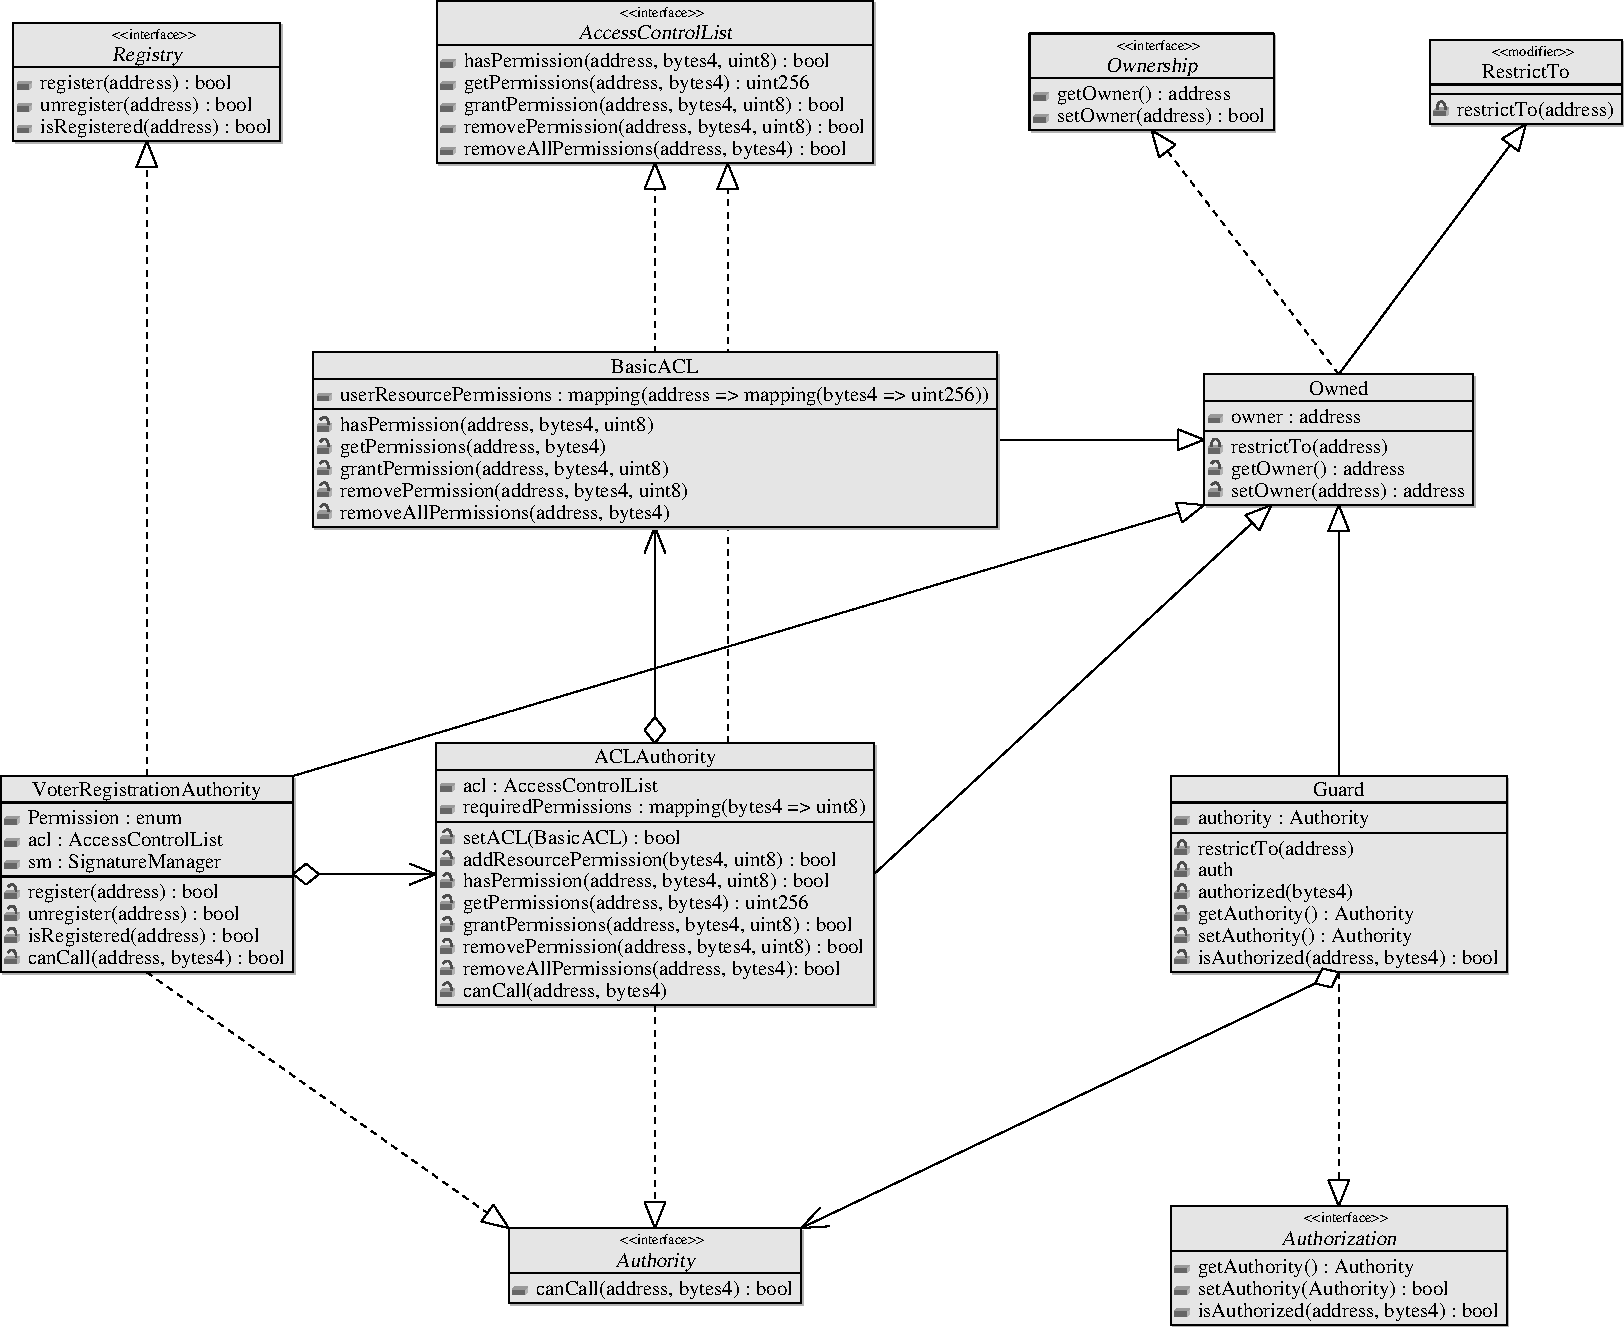
\includegraphics[width=\textwidth]{figures/authorization/figure}
  % \includestandalone[width=\textwidth]{\fig{authorization}}
\end{figure}

\subsubsection{Interface Registry}

The \solt{interface}, \sol{interface Registry}, introduces three \solt{function}
definitions required to achieve basic registry functionality:

\begin{enumerate}
  \item \sol{function register}, which \emph{registers} a \emph{subject}.

  \item \sol{function unregister}, which \emph{unregisters} a \emph{subject}.

  \item \sol{function isRegistered}, which evaluates whether a \emph{subject} is
    \emph{registered}.
\end{enumerate}

\begin{solidity}[interface Registry]
interface Registry {
  function register (address _subject) public returns (bool _success);
  function unregister (address _subject) public returns (bool _success);
  function isRegistered (address _subject) public constant returns (bool _isRegistered);
}
\end{solidity}

\begin{interface}
  \item \specification{}

  \begin{functions}
    \item \sol{function isRegistered (address _subject)}, evaluates whether some
      \emph{subject} is \emph{registered}.

      \begin{parameters}
        \item \sol{address _subject}, the \solt{address} of an account
          representing the \emph{subject}, to evaluate the \emph{registration}
          of.
      \end{parameters}

      \begin{returns}
        \item \sol{bool _isRegistered}, returns the \solt{true} if the
          \emph{subject} is \emph{registered}, otherwise \solt{false}.
      \end{returns}

    \item \sol{function unregister (address _subject)}, \emph{unregisters} a
      \emph{subject}.

      \begin{parameters}
        \item \sol{address _subject}, the account \solt{address} of the
          \emph{subject} who is to be \emph{unregistered}.
      \end{parameters}

      \begin{returns}
        \item \sol{bool _success}, resolves to \solt{true} if the operation was
          successful, otherwise \solt{false}.
      \end{returns}

    \item \sol{function register (address _subject)}, \emph{registers} a
      \emph{subject}.

      \begin{parameters}
        \item \sol{address _subject}, the account \solt{address} of the
          \emph{subject} who is to be \emph{registered}.
      \end{parameters}

      \begin{returns}
        \item \sol{bool _success}, resolves to \solt{true} if the operation was
          successful, otherwise \solt{false}.
      \end{returns}
  \end{functions}
\end{interface}


\subsubsection{Contract VoterRegistrationAuthority}

The \solt{contract}, \sol{contract VoterRegistrationAuthority}, is the final
component of our authorization design and is required to construct a generalized
voter registration authority capable of managing registered voters and
conducting elections.

% signatureMap['vote'] = bytes4(sha3('vote(uint8[],uint8[])'));
\begin{solidity}[contract VoterRegistrationAuthority]
contract VoterRegistrationAuthority is Owned, Registry, Authority {
  enum Permissions {
    Vote
  }

  AccessControlList acl;
  mapping (bytes32 => bytes4) resourceSignatures;

  constructor () public {
    acl = new ACLAuthority(true);

    resourceSignatures['vote'] = bytes4(sha3('vote()'));

    acl.setRequiredResourcePermission(
      resourceSignature('vote'),
      uint8(Permissions.Vote)
    );
  }

  function register (address _voter) public restrictTo(owner) returns (bool _success) {
    return acl.grantPermission(_voter, resourceSignatures['vote'], uint8(Permissions.Vote));
  }

  function unregister (address _voter) public restrictTo(owner) returns (bool _success) {
    return acl.revokePermission(_voter, resourceSignatures['vote'], uint8(Permissions.Vote));
  }

  function isRegistered (address _voter) public constant returns (bool _isRegistered) {
    return acl.hasPermission(_voter, resourceSignatures['vote'], uint8(Permissions.Vote));
  }

  function canCall (address _subject, bytes4 _resource) public constant returns (bool _canCall) {
    return acl.canCall(_subject, _resource);
  }
}
\end{solidity}

\todo{Finish documenting the VoterRegistrationAuthority implementation.}

\begin{state}
  \item \attributes

  \begin{public}
    \item \sol{AccessControlList acl} maintains the \solt{address} of an ACL
      implementation, a \solt{contract} which implements \sol{interface
      AccessControlList}.

    \item \sol{mapping (bytes32 => bytes4) resourceSignatures} maintains a
      mapping of strings, \sol{bytes32}, to \solt{function} signature,
      \sol{bytes4}.
  \end{public}
\end{state}

\begin{code}
  \item \operations

  \begin{constructor}
    \item \sol{constructor (bool _createACL)}, upon creation and initialization
      of this \solt{contract} the \solt{constructor} can deploy a
      \solt{contract}, \sol{contract BasicACL}, if the \solt{bool}, \sol{bool
      _createACL}, is set to \solt{true}.

      \begin{parameters}
      \item \sol{bool _createACL}, set to \solt{true} to deploy an ACL
        implementation, \sol{contract BasicACL}, in addition to this
        \solt{contract}; otherwise \solt{false}.
      \end{parameters}
  \end{constructor}

  \begin{functions}
    \item \sol{function setAcl (AccessControlList _acl)}, updates the
      \solt{contract} reference which is responsible for managing ACL requests.

      \begin{modifiers}
        \item \sol{modifier restrictTo (owner)}, restricts access to the
          \solt{function} such that \emph{only} the current \solt{owner} of the
          \sol{contract} can call it.
      \end{modifiers}

      \begin{parameters}
        \item \sol{AccessControlList _acl}, the ACL implementation which access
          control responsibilities are to be delegated to.
      \end{parameters}

      \begin{returns}
        \item \sol{bool _success}, resolves to \solt{true} if the operation was
          successful, otherwise \solt{false}.
      \end{returns}


    \item \sol{function setRequiredResourcePermission (bytes4 _resource, uint8 _permission)},
      updates the mapping representing the \emph{permission} required to access
      some \emph{resource}, \solt{function} signature.

      \begin{modifiers}
        \item \sol{modifier restrictTo (owner)}, restricts access to the
          \solt{function} such that \emph{only} the current \solt{owner} of the
          \sol{contract} can call it.
      \end{modifiers}

      \begin{parameters}
        \item \sol{bytes4 _resource}, the \emph{resource}, \solt{function}
          signature, which the \emph{permission} is to be modified for.

        \item \sol{uint8 _permission}, a \solt{uint8} value representing the
          \emph{permission-bit} required for the \emph{resource}.
      \end{parameters}

      \begin{returns}
        \item \sol{bool _success}, resolves to \solt{true} if the operation was
          successful, otherwise \solt{false}.
      \end{returns}


    \item \sol{function canCall (address _subject, bytes4 _resource)}, evaluates
      whether a \emph{subject} can access to some \emph{resource} by validating
      with the ACL implementation that the \emph{subject} has the required
      \emph{resource} \emph{permission}.

      \begin{parameters}
        \item \sol{address _subject}, the \emph{subject}, Ethereum account,
          whose \emph{permissions} are being evaluated.

        \item \sol{bytes4 _resource}, the \emph{resource}, \solt{contract
          function}, which the \emph{subject's} \emph{permissions} are being
          evaluated against.
      \end{parameters}

      \begin{returns}
        \item \sol{bool _canCall}, resolves to \solt{true} if the
          \emph{subject}, \sol{address _subject}, is permitted to access the
          \emph{resource}, \sol{bytes4 _resource}, otherwise \solt{false}.
      \end{returns}


    \item
      \sol{function hasPermission (address _subject, bytes4 _resource, uint8 _permission)}, \\
      \sol{function getPermissions (address _subject, bytes4 _resource)}, \\
      \sol{function setPermissions (address _subject, bytes4 _resource, uint256 _permissions)}, \\
      \sol{function grantPermission (address _subject, bytes4 _resource, uint8 _permission)}, \\
      \sol{function revokePermission (address _subject, bytes4 _resource, uint8 _permission)}, \\
      all ACL responsibilities originating from \sol{interface AccessControlList}
      are delegated to the provided ACL implementation stored in
      \sol{AccessControlList acl}.

      \begin{modifiers}
        \item \sol{modifier restrictTo (owner)}, restricts access to the
          \solt{function} such that \emph{only} the current \solt{owner} of the
          \solt{contract} can call this \solt{function}; this applies to
          \solt{function}[s] \sol{setPermissions}, \sol{grantPermission}, and
        \sol{revokePermission}.
      \end{modifiers}
  \end{functions}
\end{code}



% Section: Election Components
% \section{Election Components}

This section explores the components relating to elections; election contracts:

\begin{enumerate}
  \item \emph{First-Past-the-Post},
  \item \emph{Range Vote}, and
  \item \emph{Single Transferable Vote}.
\end{enumerate}

% \begin{figure}[H]
%   \centering
%   \caption{Authorization dependency graph modeling.}% \label{fig:authorization}
%   \figurepdf[width=\textwidth]{authorization}
%   % 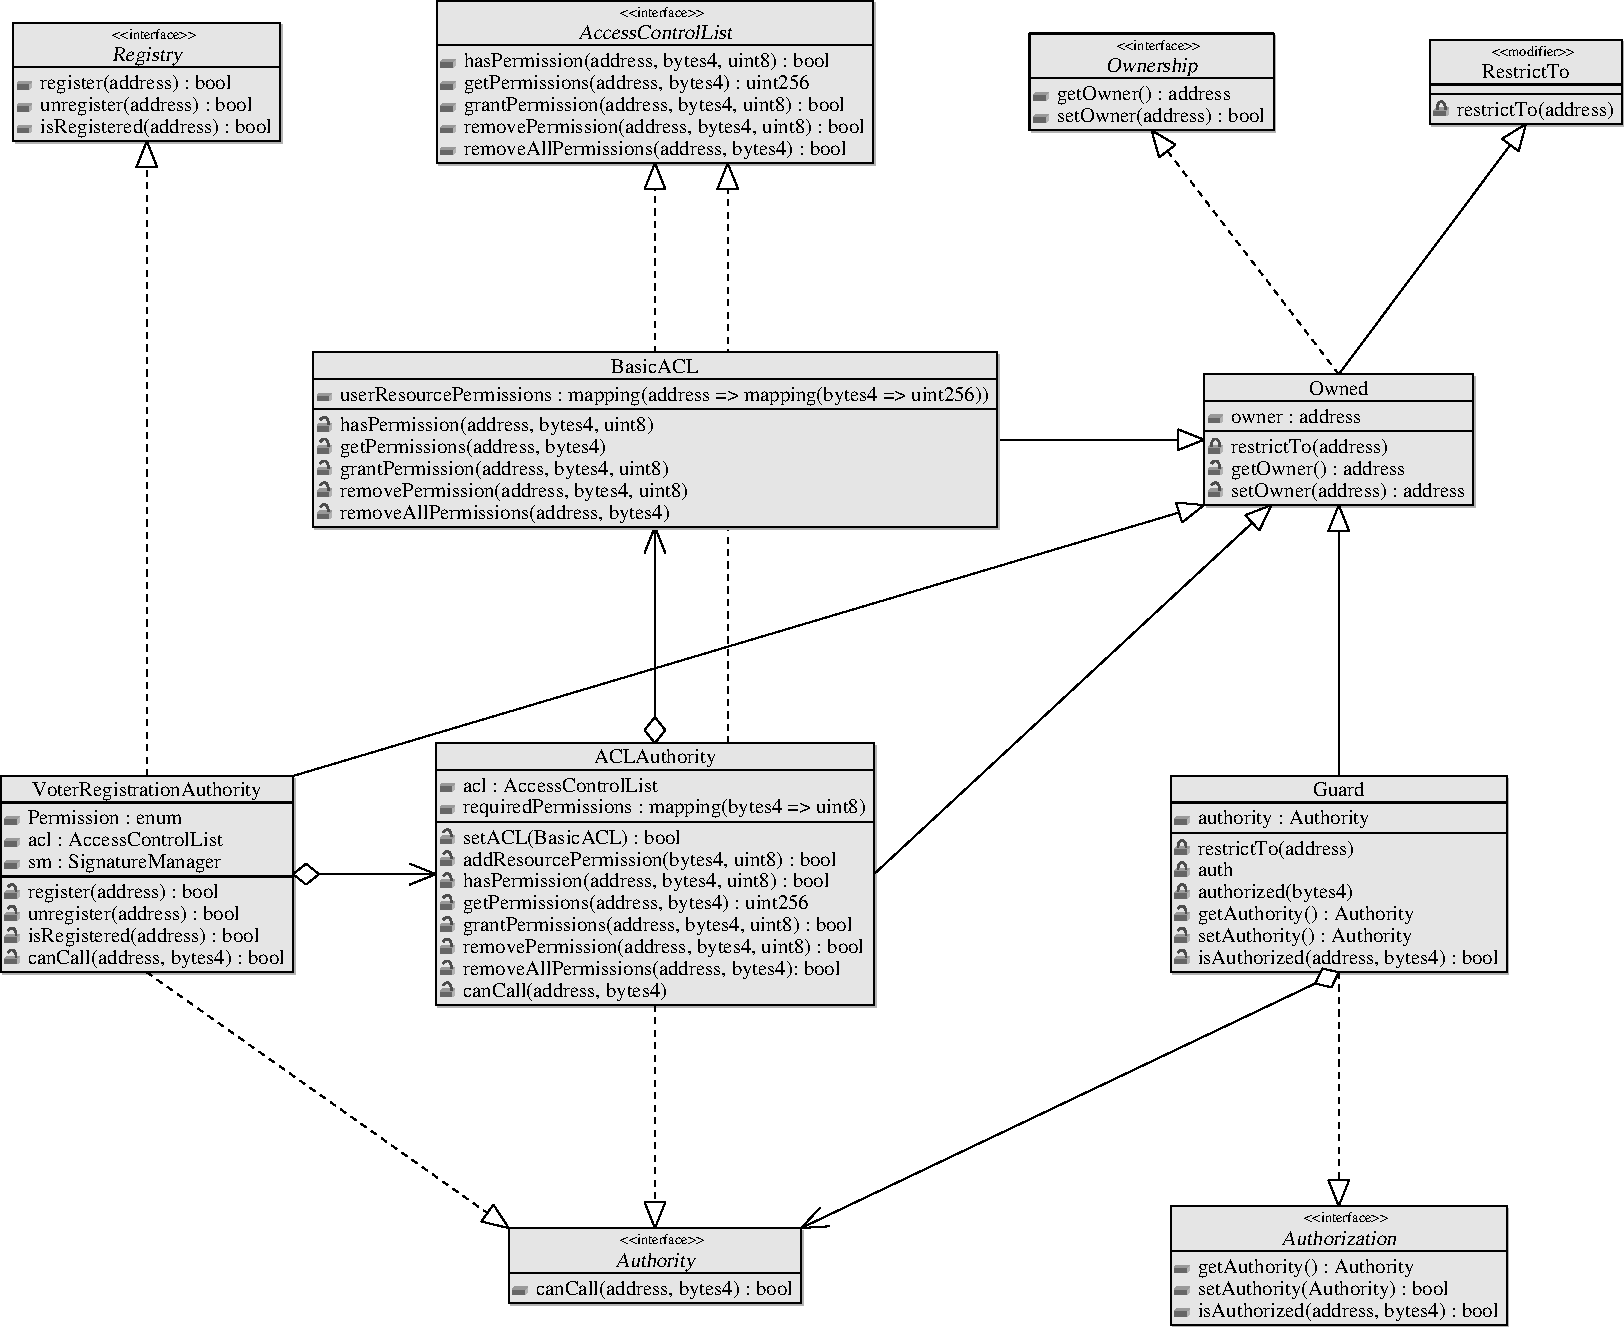
\includegraphics[width=\textwidth]{figures/authorization/figure}
%   % \includestandalone[width=\textwidth]{\fig{authorization}}
% \end{figure}

% \subsection{Finite State Machine}

% \subsection{First-Past-the-Post}
% The first-past-the-post \solt{contract} is the simplest election \solt{contract}
% implementation.

\subsection{Election Contracts}

\subsubsection{Contract FirstPastThePost}

The first-past-the-post \solt{contract} is the simplest election \solt{contract}
implementation.

\begin{solidity}[contract FirstPastThePost]
contract FirstPastThePost is Owned, Guard {
  uint public creationTime = now;

  Choice[] public choices;
  mapping(address => bool) public voted;
  Choice public winner;

  enum Phase { Configuration, Frozen, Vote, Tally }

  struct PhaseProperties {
    Phase phase;
    uint startTime;
    uint endTime;
    Phase nextPhase;
  }

  mapping (Phase => PhaseProperties) phases;
  Phase public phase = Phase.Configuration;

  constructor () {
    phases[Phase.Configuration] = PhaseProperties({
      phase: Phase.Configuration,
      start_time: now,
      end_time: 0,
      next_phase: Phase.Configuration
    });
  }

  // This is the current phase.
  uint public freezeTime;

  // Start and end time for the election.
  uint public voteStartTime;
  uint public voteEndTime;

  // This is a type for a single proposal.
  struct Choice {
    // Short name (up to 32 bytes).
    bytes32 name;

    // TODO: choice description?
    // bytes32 description;

    // Number of accumulated votes.
    uint40 voteCount;
  }

  // Restrict calls to _account.
  modifier restrictTo(address _account) {
    require(msg.sender == _account);
    _;
  }

  // Check current stage.
  modifier atPhase(Phase _phase) {
    require(phase == _phase);
    _;
  }

  // This modifier goes to the next phase after the function is done.
  modifier transitionNextPhase() {
    _;
    nextPhase();
  }

  // Move into next phase.
  function nextPhase() internal {
    phase = Phase(uint(phase) + 1);
  }

  // Perform timed transitions. Be sure to mention this modifier first,
  // otherwise the guards will not take the new stage into account.
  modifier timedTransitions() {
    if (phase == Phase.Frozen && now >= voteStartTime)
      nextPhase();
    if (phase == Phase.Vote && now >= voteEndTime)
      nextPhase();
    // The other stages transition by transaction
    _;
  }

  /* Election Functions */
  // Freeze the configuration.
  function freeze() restrictTo(owner) atPhase(Phase.Configuration) transitionNextPhase {
    require(voteStartTime > now);
    require(choices.length > 1);
    freezeTime = now;
    delete owner;
  }

  // Cast a ballot.
  function vote(uint8 choice) timedTransitions atPhase(Phase.Vote) {
    // Each address can only vote once.
    require(!voted[msg.sender]);
    voted[msg.sender] = true;

    choices[choice].voteCount += 1;
  }

  // Tally ballots.
  function tally() timedTransitions atPhase(Phase.Tally) {
    winner = choices[0];
    for (uint8 i = 0; i < choices.length; i++) {
      if (choices[i].voteCount > winner.voteCount)
        winner = choices[i];
    }
  }

  /* Configuration Functions */
  constructor () {}

  function setVoteStartTime(uint _voteStartTime) atPhase(Phase.Configuration) restrictTo(owner) {
    voteStartTime = _voteStartTime;
  }

  function setVoteEndTime(uint _voteEndTime) atPhase(Phase.Configuration) restrictTo(owner) {
    voteEndTime = _voteEndTime;
  }

  function addChoices(bytes32[] _choices) atPhase(Phase.Configuration) restrictTo(owner) {
    for (uint i = 0; i < _choices.length; i++) {
      choices.push(Choice({
        name: _choices[i],
        voteCount: 0
      }));
    }
  }

  function addChoice(bytes32 _name) atPhase(Phase.Configuration) restrictTo(owner) {
    choices.push(Choice({
      name: _name,
      voteCount: 0
    }));
  }

  //   function modifyChoice(uint8 key, bytes32 _name)
  //     atPhase(Phase.Configuration)
  //     restrictTo(owner)
  //   {
  //     require(key < choices.length-1);
  //
  //     choices[key] = Choice({
  //       name: _name,
  //       voteCount: 0
  //     });
  //   }
}
\end{solidity}

\begin{state}
  \item \attributes

  \begin{public}
    \item \sol{AccessControlList choices} maintains the \solt{address} of an ACL
      implementation, a \solt{contract} which implements \sol{interface
      AccessControlList}.

    \item \sol{mapping (bytes4 => uint8) requiredResourcePermissions} maintains a
      mapping of \solt{function}[s], \sol{bytes4}, to required
      \emph{permission}, \sol{uint8}.
  \end{public}
\end{state}

\begin{code}
  \item \operations

  \begin{constructor}
    \item \sol{constructor (bool _createACL)}, upon creation and initialization
      of this \solt{contract} the \solt{constructor} can deploy a
      \solt{contract}, \sol{contract BasicACL}, if the \solt{bool}, \sol{bool
      _createACL}, is set to \solt{true}.

      \begin{parameters}
      \item \sol{bool _createACL}, set to \solt{true} to deploy an ACL
        implementation, \sol{contract BasicACL}, in addition to this
        \solt{contract}; otherwise \solt{false}.
      \end{parameters}
  \end{constructor}

  \begin{functions}
    \item \sol{function setAcl (AccessControlList _acl)}, updates the
      \solt{contract} reference which is responsible for managing ACL requests.

      \begin{modifiers}
        \item \sol{modifier restrictTo (owner)}, restricts access to the
          \solt{function} such that \emph{only} the current \solt{owner} of the
          \sol{contract} can call it.
      \end{modifiers}

      \begin{parameters}
        \item \sol{AccessControlList _acl}, the ACL implementation which access
          control responsibilities are to be delegated to.
      \end{parameters}

      \begin{returns}
        \item \sol{bool _success}, resolves to \solt{true} if the operation was
          successful, otherwise \solt{false}.
      \end{returns}


    \item \sol{function setRequiredResourcePermission (bytes4 _resource, uint8 _permission)},
      updates the mapping representing the \emph{permission} required to access
      some \emph{resource}, \solt{function} signature.

      \begin{modifiers}
        \item \sol{modifier restrictTo (owner)}, restricts access to the
          \solt{function} such that \emph{only} the current \solt{owner} of the
          \sol{contract} can call it.
      \end{modifiers}

      \begin{parameters}
        \item \sol{bytes4 _resource}, the \emph{resource}, \solt{function}
          signature, which the \emph{permission} is to be modified for.

        \item \sol{uint8 _permission}, a \solt{uint8} value representing the
          \emph{permission-bit} required for the \emph{resource}.
      \end{parameters}

      \begin{returns}
        \item \sol{bool _success}, resolves to \solt{true} if the operation was
          successful, otherwise \solt{false}.
      \end{returns}


    \item \sol{function canCall (address _subject, bytes4 _resource)}, evaluates
      whether a \emph{subject} can access to some \emph{resource} by validating
      with the ACL implementation that the \emph{subject} has the required
      \emph{resource} \emph{permission}.

      \begin{parameters}
        \item \sol{address _subject}, the \emph{subject}, Ethereum account,
          whose \emph{permissions} are being evaluated.

        \item \sol{bytes4 _resource}, the \emph{resource}, \solt{contract
          function}, which the \emph{subject's} \emph{permissions} are being
          evaluated against.
      \end{parameters}

      \begin{returns}
        \item \sol{bool _canCall}, resolves to \solt{true} if the
          \emph{subject}, \sol{address _subject}, is permitted to access the
          \emph{resource}, \sol{bytes4 _resource}, otherwise \solt{false}.
      \end{returns}


    \item
      \sol{function hasPermission (address _subject, bytes4 _resource, uint8 _permission)}, \\
      \sol{function getPermissions (address _subject, bytes4 _resource)}, \\
      \sol{function setPermissions (address _subject, bytes4 _resource, uint256 _permissions)}, \\
      \sol{function grantPermission (address _subject, bytes4 _resource, uint8 _permission)}, \\
      \sol{function revokePermission (address _subject, bytes4 _resource, uint8 _permission)}, \\
      all ACL responsibilities originating from \sol{interface AccessControlList}
      are delegated to the provided ACL implementation stored in
      \sol{AccessControlList acl}.

      \begin{modifiers}
        \item \sol{modifier restrictTo (owner)}, restricts access to the
          \solt{function} such that \emph{only} the current \solt{owner} of the
          \solt{contract} can call this \solt{function}; this applies to
          \solt{function}[s] \sol{setPermissions}, \sol{grantPermission}, and
        \sol{revokePermission}.
      \end{modifiers}
  \end{functions}
\end{code}


\subsubsection{Range Vote}

\subsubsection{Single Transferable Vote}


% Section: Delegation Components
% \section{Delegation Components}

This section explores the components relating to vote delegation. The delegation
components are responsible for managing the delegation of voters' votes to
delegates.

% \begin{figure}[H]
%   \centering
%   \caption{Authorization dependency graph modeling.}% \label{fig:authorization}
%   \figurepdf[width=\textwidth]{authorization}
%   % 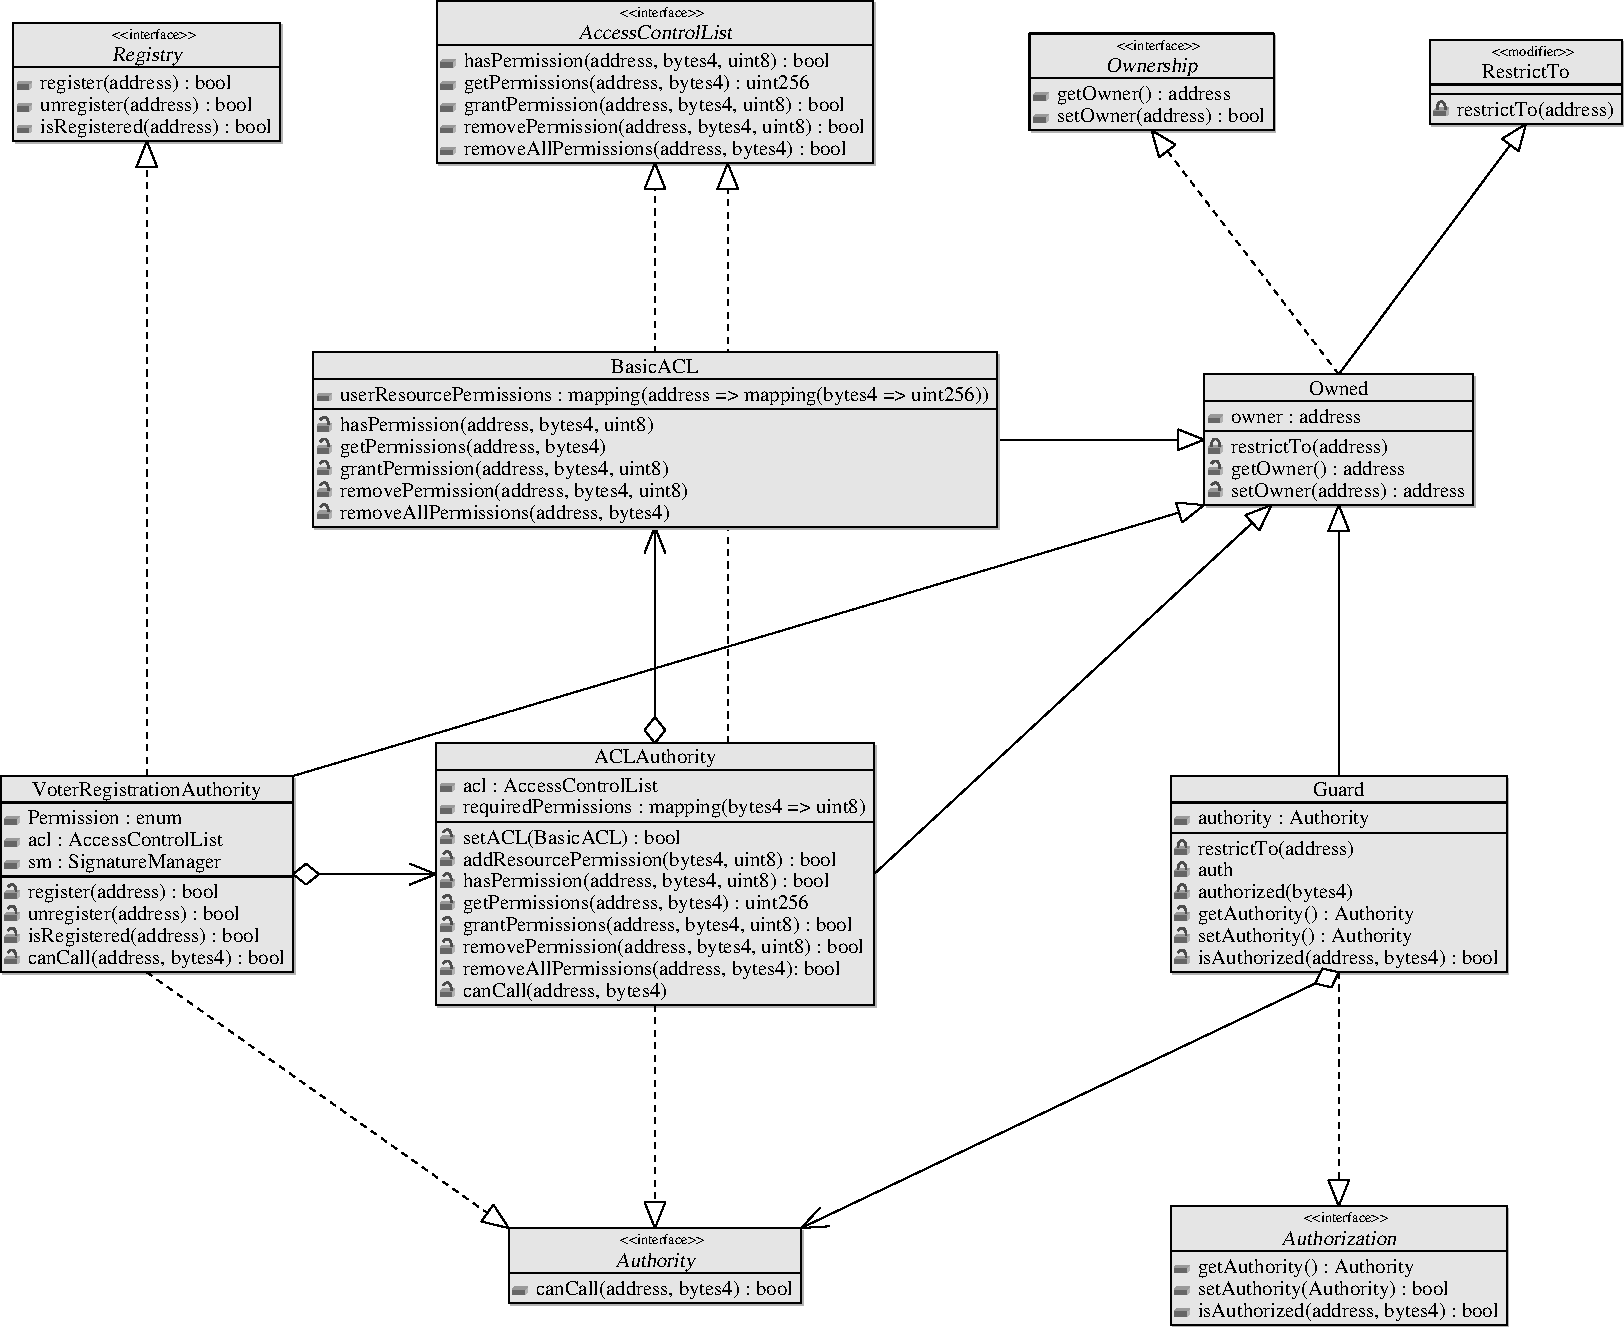
\includegraphics[width=\textwidth]{figures/authorization/figure}
%   % \includestandalone[width=\textwidth]{\fig{authorization}}
% \end{figure}

% Section: delegation
\subsection{Delegation Contracts}

\begin{solidity}[Vote Delegation]
mapping (address => Voter) voters;

function delegateVote (address delegate) public auth returns (bool _success) {
  // The `auth` modifier prevents this function from being
  // called until the Authority has confirmed that the
  // the message sender has the proper privileges.
  Voter cursor;
  uint40 weight = voters[msg.sender].weight;

  // Cycle Detection
  mapping (address => bool) visited;
  visited[msg.sender] = true;
  visited[delegate] = true;

  cursor = voters[delegate];
  while (cursor.delegate) {
    address newDelegate = cursor.delegate;
    if (visited[newDelegate]) return false;
    cursor = voters[newDelegate];
    visited[newDelegate] = true;
  }

  // Decrement weights of old delegate chain.
  cursor = voters[msg.sender];
  while (cursor.delegate) {
    address newDelegate = cursor.delegate;
    cursor = voters[newDelegate];
    cursor.weight -= weight;
  }

  // Increment weights of new delegate chain.
  cursor = voters[msg.sender];
  cursor.delegate = delegate;
  while (cursor.delegate) {
    address newDelegate = cursor.delegate;
    cursor = voters[newDelegate];
    cursor.weight += weight;
  }

  return true;
}
\end{solidity}


